\documentclass[8pt, a4paper]{extarticle}
\usepackage{amsmath}
\usepackage{amssymb}
\usepackage{mathtools}
\usepackage{multicol}
\usepackage{enumitem}
\usepackage{mathrsfs}
\usepackage{booktabs}
\usepackage{tikz}


\usepackage{xcolor}
\usepackage{graphicx}
\graphicspath{ {./images/} }

\usepackage[
    landscape,
    margin=0.8cm,
    footskip=0.5cm
]{geometry}

\usepackage[
    skip=5pt plus1pt,
    indent=0pt
]{parskip}

\usepackage[
    compact
]{titlesec}

\usepackage[hidelinks]{hyperref}

\title{Analysis I FS26}
\author{Elias Gerber}
\date{}

\AtBeginDocument{
  \setlength\abovedisplayskip{0pt}
  \setlength\belowdisplayskip{0pt}
  \setlength\abovedisplayshortskip{-\baselineskip}
  \setlength\belowdisplayshortskip{0pt}
}

\setlist{noitemsep, topsep=0pt, parsep=0pt, partopsep=-0.6\parskip}

\newlength{\sepwidth}
\setlength{\sepwidth}{0.4pt}
\setlength{\columnseprule}{\sepwidth}

\newcommand{\secsep}{
    \vspace{\baselineskip}
    \leaders
        \hrule width \columnwidth \relax
    \vskip\sepwidth
}

% Pastel-Palette, wird bei jedem Header weitergeschaltet, damit aufeinanderfolgende
% Sections/Subsections unterschiedliche Farben haben
\definecolor{pastelRed}{RGB}{255,179,186}
\definecolor{pastelOrange}{RGB}{255,223,186}
\definecolor{pastelYellow}{RGB}{255,255,186}
\definecolor{pastelGreen}{RGB}{186,255,201}
\definecolor{pastelTeal}{RGB}{186,255,255}
\definecolor{pastelBlue}{RGB}{186,225,255}
\definecolor{pastelPurple}{RGB}{223,186,255}
\definecolor{pastelPink}{RGB}{255,186,240}

% \ifcase resolves only a plain colour name (never \colorbox directly), since
% \colorbox waiting on an argument across an \ifcase/\fi boundary corrupts TeX's
% conditional stack; \colorbox itself is then called once, fully outside \ifcase.
\newcounter{seccolor}
\newcommand{\currentseccolor}{%
    \ifcase\value{seccolor}\relax
        pastelRed%
    \or pastelRed%
    \or pastelOrange%
    \or pastelYellow%
    \or pastelGreen%
    \or pastelTeal%
    \or pastelBlue%
    \or pastelPurple%
    \or pastelPink%
    \fi
}
\newcommand{\seccolorbox}{%
    \stepcounter{seccolor}%
    \ifnum\value{seccolor}>8 \setcounter{seccolor}{1}\fi
    \colorbox{\currentseccolor}%
}

% (Sub)subsections reuse the enclosing section's colour rather than cycling on
% their own, so every header within a section matches
\newcommand{\subseccolorbox}{\colorbox{\currentseccolor}}

\titleformat{\section}
    {\secsep\normalfont\Large\bfseries}
    {}
    {0pt}
    {\seccolorbox}

\titleformat{\subsection}
    {\normalfont\large\bfseries}
    {}
    {0pt}
    {\subseccolorbox}

\titleformat{\subsubsection}
    {\normalfont\normalsize\bfseries}
    {}
    {0pt}
    {\subseccolorbox}

\newcommand{\key}[1]{\textbf{\textit{\color{red}{#1}}}}

\setcounter{secnumdepth}{1}
\numberwithin{equation}{section}
\DeclareMathOperator{\sgn}{sgn}

\newcommand{\NN}{\mathbb{N}}
\newcommand{\ZZ}{\mathbb{Z}}
\newcommand{\QQ}{\mathbb{Q}}
\newcommand{\RR}{\mathbb{R}}
\newcommand{\CC}{\mathbb{C}}

\newcommand{\DD}{\mathbb{D}}
\newcommand{\WW}{\mathbb{W}}

\newcommand{\Def}{\paragraph{Def.}}
\newcommand{\Satz}{\paragraph{Satz}}
\newcommand{\Kor}{\paragraph{Kor.}}
\newcommand{\Bsp}{\paragraph{Bsp.}}
\newcommand{\Bew}{\paragraph{Bew.}}
\newcommand{\Tab}{\paragraph{Tabelle}}
\newcommand{\Bild}{\paragraph{Bild}}

\begin{document}

\begin{multicols*}{3}

    {\large \textbf{Analysis I FS26}}
    Elias Gerber

    Abschnitte mit $\star$ stammen nicht unbedingt aus Skript oder Slides.

    W\section{1. Logik, Mengen, Zahlen}
\subsection{Logik}

\Def Eine \key{math. Aussage} ist entweder wahr oder falsch

\Def \key{Prädikat} ist Aussage mit Variablen: $A(x)$ oder $A(x, y, \ldots)$ 

\Def \key{Verneinung} (Negation) einer math. Aussage ist $\lnot A$.

\Def Wir führen die folgenden \key{Quantoren} (”Kurzschreibweisen”) ein:
$\forall$, $\exists$, $\exists!$, $\nexists$. 
Quantoren stehen vor den Aussagen.

\Def Wir führen die folgenden \key{Grundverknüpfungen} ein:
$\land$, $\lor$, $\implies$, $\iff$.

\Satz Es gelten die folgenden Regeln
\vspace{-0.6em}
\begin{itemize}
    \item $\lnot \forall x \, A(x) \, \iff \, \exists x \, \lnot A(x)$
    \item $\lnot \exists x \, A(x) \, \iff \, \forall x \, \lnot A(x)$
    \item $\forall x (A(x) \, \land \, B(x)) \, \iff \, (\forall x A(x)) \, \land \, (\forall x \, B(x))$
    \item $\exists x (A(x) \, \lor \, B(x)) \, \iff \, (\exists x A(x)) \, \lor \, (\exists x \, B(x))$
    \item $\exists x (A(x) \, \land \, B(x)) \, \implies \, (\exists x A(x)) \, \land \, (\exists x \, B(x))$ \hspace{10pt} $\star$
\end{itemize}

\subsection{Mengen}

\Def \key{Menge} ist eine Ansammlung von  Elementen, entweder aufgelistet
oder durch Eigenschaften charakterisiert.

\key{Leere Menge}: $\varnothing$. Element $x$ in Menge $M$: $x \in M$. Andernfalls: $x \notin M$.

\Def Seinen $X$ und $Y$ zwei Mengen:
\vspace{-0.6em}
\begin{itemize}
    \item \key{Teilmenge} $X \subset Y$ oder $X \subseteq Y$: $\forall x \in X : x \in Y$
    \item \key{echte Teilmenge} $X \subsetneq Y$: $(X \subset Y) \, \land \, (X\ne Y)$
    \item \key{Komplement} Falls $X \subset Y$ gilt, ist $X^c := \{y \, | \, y \in Y \, \land \, y \notin X\}$
\end{itemize}

\Def Mit Mengen folgende \key{Operationen}:
$\cup$, $\cap$, $\backslash$, $\times$.

\subsection{Zahlen}

\Def \key{Zahlmengen}: $\NN = \{1, 2, \ldots\}$, $\NN_0 = \NN \cup \{0\} = \{0, 1, 2, \ldots\}$, $\ZZ$, $\QQ$, $\RR$.
Wir betrachten oft auch: $\RR^+ = (0, \infty)$, $\RR^+_0 = [0, \infty)$, $\RR^-$, $\RR^-_0$

\Satz \key{Theorem von Aaron}: In $\NN$, oder auch in $\RR$, gilt: $1 + 1 = 2$.

\Def \key{Intervalle}, $I \subset \RR$:
offenes Intervall $(a, b)$, abgeschlossenes Intervall $[a, b]$ und halboffene Intervalle $[a, b)$ $(a, b]$

$\RR = (-\infty, \infty)$, $a, b \in \RR$ \key{beschränktes Int.},
$(-\infty, b) = \{x \in \RR \, | \, x < b\}$

\Def \key{Kenngrössen} von Teilmengen $X \subset \RR$:
\vspace{-0.6em}
\begin{itemize}
    \item \key{obere Schranke} ist $y \in \RR$ mit $\forall x \in X : x\le y$
    \item \key{untere Schranke} ist $y \in \RR$ mit $\forall x \in X : y\le x$
    \item \key{Maximum} ist $x_0 \in X$ mit $\forall x \in X : x\le x_0$
    \item \key{Minimum} ist $x_0 \in X$ mit $\forall x \in X : x_0\le x$
    \item \key{Supremum} ist kleinste obere Schranke von $X$, $\sup(X)$
    \item \key{Infimum} ist grösste untere Schranke von $X$, $\inf(X)$
\end{itemize}

\Satz
Es gelten die folgenden Tatsachen:
\vspace{-0.6em}
\begin{itemize}
    \item Maximum und Minimum eindeutig - sofern sie existieren
    \item $M\ne \varnothing$, nach unten/oben beschr. hat eindeutig $\inf(M)$/$\sup(M)$.
    \item $S = \sup(X)$ wenn $(\forall x \in X : x\le S) \, \land \, (\forall \varepsilon > 0 \, \exists x \in X : x > S - \varepsilon)$
    \item $I = \inf(X)$ wenn $(\forall x \in X : I\le x) \, \land \, (\forall \varepsilon > 0 \, \exists x \in X : x < I + \varepsilon)$
\end{itemize}

\Def Axiome von $\RR$:
\vspace{-0.6em}
\begin{itemize}
    \item \key{Axiome der Addition}:
    \begin{itemize}
        \item[(A1)] $x + (y + z) = (x + y) + z$ (Assoziativität)
        \item[(A2)] $x + 0 = x$ (neutrales Element)
        \item[(A3)] $x + (-x) = 0$ (inverses Element)
        \item[(A4)] $x + y = y + x$ (Kommutativität) 
    \end{itemize}

    \item \key{Axiome der Multiplikation}:
    \begin{itemize}
        \item[(M1)] $x \cdot (y \cdot z) = (x \cdot y) \cdot z$ (Assoziativität)
        \item[(M2)] $x \cdot 1 = x$ (neutrales Element)
        \item[(M3)] $x \cdot x^{-1} = 1$ (inverses Element)
        \item[(M4)] $x \cdot y = y \cdot x$ (Kommutativität)
    \end{itemize}
    
    \item \key{Distributivitätsgesetz} (Kompatibilität von Addition und Multiplikation):
        $x \cdot (y + z) = x \cdot y + x \cdot z = (y + z) \cdot x$
    
    \item \key{Ordnungsaxiome}:
    \begin{itemize}
        \item[(O1)] $x\le x$ (Reflexivität)
        \item[(O2)] $(x\le y \, \land \, y\le z) \implies (x\le z)$ (Transitivität)
        \item[(O3)] $(x\le y \, \land \, y\le x) \implies (x = y)$ (Antisymmetrie)
        \item[(O4)] $(x\le y$ oder $y\le x)$ (Totalität)
    \end{itemize}

    \item \key{Konsistenz mit Addition und Multiplikation}:
    \item \begin{itemize}
        \item[(K1)] $x\le y \implies x + z\le y + z$
        \item[(K2)] $(x\ge 0 \, \land \, y\ge 0) \implies x \cdot y\ge 0$
    \end{itemize}
\end{itemize}

\Satz Ordnungsvollständigkeit: $A, B \subset \RR$, $A\ne \varnothing$, $B\ne \varnothing$,
$\forall a \in A \, \forall b \in B : a\le b$: \\
Es gibt $c \in \RR$ so dass $\forall a \in A : a\le c$ und $\forall b \in B : c\le b$

\Satz $\RR$ ist ein geordneter und ordnungsvollständiger Körper

\Kor Eigenschaften von $\RR$
\vspace{-0.6em}
\begin{itemize}
    \item Additive und multiplikative Inverse sind eindeutig bestimmt
    \item $0 \cdot x = 0$
    \item $-1 \cdot x = -x$
    \item $y\ge 0 \iff -y\le 0$
    \item $y^2\ge 0$
    \item Aus $x\le y$ und $u\le v$ folgt $x + u\le y + v$
    \item Falls $0\le x\le y$ und $u\ge 0$, $x \cdot u\le y \cdot u$
\end{itemize}

\Kor \key{Archimedisches Prinzip}
\vspace{-0.6em}
\begin{itemize}
    \item Für $x \in \RR$ und $y > 0$ existiert $n \in \NN$ mit $n \cdot y\ge x$
    \item Für jedes $\varepsilon > 0$ existiert $n \in \NN$ mit $\frac{1}{n}\le \varepsilon$
\end{itemize}

\Def $\max\{x, y\}$, $\min\{x, y\}$, \key{Absolutbetrag} $|x| = \max\{x, -x\}$

\Satz \key{Satz von Chris}: Für $a, b, c \in \RR$ gilt $a \cdot (b + c) = a \cdot b + a \cdot c$

\Satz \key{Eigenschaften des Absolutbetrags}
\vspace{-0.6em}
\begin{itemize}
    \item $|x|\ge 0$
    \item $|x + y|\le |x| + |y|$ (\key{Dreiecksungleichung})
    \item $|x + y|\ge ||x| - |y||$
\end{itemize}

\Satz \key{Youngsche Ungleichung}: Für jedes $\varepsilon > 0$ und $x, y \in \RR$ gilt:
$$2|xy|\le \varepsilon x^2 + \frac{1}{\varepsilon}y^2$$

\subsection{Vektoren und Vektorräume}

\Def Für $x, y \in \RR^n$:
\vspace{-0.6em}
\begin{itemize}
    \item \key{(Standard-)Skalarprodukt}: $x \cdot y = <x,y> = [x,y] := \sum_{i=1}^{n}x_i y_i$
    \item \key{Euklidische Norm}: $||x|| := \sqrt{\sum_{i=1}^{n}x_i^2}$
    \item \key{Euklidischer Abstand}: $d(x,y) := \sqrt{\sum_{i=1}^{n}(x_i-y_i)^2}$
\end{itemize}

\Satz \key{Dreiecksungleichung}: $\forall x,y,z \in \RR^n : ||x-z||\le ||x-y|| + ||y - z||$

\subsection{Komplexe Zahlen}

\Def \key{komplexe Zahlen}: $\CC = \{z = a + ib \, | \, a,b \in \RR\}$.
$z = a + ib$ heisst Normal-/aritmetische/kartesische Form. $a = Re(z)$ \key{Realteil},
$b = Im(z)$ \key{Imaginärteil}, $i^2 = -1$ \key{imag.}/\key{komplexe Einheit}. $z = ib$ ist \key{rein imaginär}

\Def $z = x + iy$ und $\overline{z} = x - iy$ sind \key{komplex konjugiert}

\Satz $\frac{z}{w} = \frac{z \cdot \overline{w}}{w \cdot \overline{w}} = \frac{z \cdot \overline{w}}{|w|^2}$
und $\overline{\frac{z}{w}} = \frac{\overline{z}}{\overline{w}}$ für $z,w \in \CC$

\Satz Eigenschaften der komplex konjugierten Zahl
\vspace{-0.6em}
\begin{itemize}
    \item $z \cdot \overline{z} = |z|^2$
    \item $z + \overline{z} = 2 Re(z)$ und $z - \overline{z} = 2iIm(z)$
    \item $\overline{\overline{z}} = z$
    \item $\overline{z \pm w} = \overline{z} \pm \overline{w}$
    \item $\overline{z \cdot w} = \overline{z} \cdot \overline{w}$
    \item $z = \overline{z}$ falls $z \in \RR$
    \item $\overline{z} = -z$ falls $z$ rein imaginär
\end{itemize}

\Def \key{Betrag} $|z| = \sqrt{a^2 + b^2}$,
\key{Abstand} $d = |z_2 - z_1| = |z_1 - z_2|$

\Satz \key{Dreiecksungleichung}: Für $z, w \in \CC$ gilt $|z + w|\le |z| + |w|$

\Satz \key{Eulersche Formel}: $e^x = \sum_{k=0}^{\infty}\frac{1}{k!}x^k$ und mit $x = it$:
$$e^{it} = \cos(t) + i\sin(t)$$

\Kor $\cos(t) = \frac{e^{it} + e^{-it}}{2}$ und $\sin(t) = \frac{e^{it} - e^{-it}}{2i}$

\Def $\cosh(t) = \frac{e^t + e^{-t}}{2}$ und $\sinh(t) = \frac{e^t - e^{-t}}{2}$

\Def \key{Polardarstellung}: $z = r \cdot e^{i\varphi}$ und $r = |z|$, $\varphi = \arg(z) \in (-\pi, \pi]$

\Satz \key{Wurzeln in $\CC$}: $z^n = re^{i\varphi}$: 
$z_k = r^{\frac{1}{n}}e^{i\frac{\varphi + 2k\pi}{n}}$ wobei $0\le k < n$

\Satz \key{Fundamentalsatz der Algebra}: $p(z) = \sum_{k=0}^{n} a_k z^k$, $a_k \in \CC$
kann als $p(z) = a_n\prod_{k=1}^{n}(z-z_k)$ geschrieben werden, wobei $z_k$ die Nullstellen
von $p(z)$ (mit Vielfachheit) sind

\Satz $p(z)$ mit $a_k \in \RR$ $\implies$ Nullstellen komplex konjugiert % SW 1, 2
    \section{2. Folgen}
\Def \key{Folge} $(a_n)_{n \in \NN_0}$, $(a_n)_{n\ge 0}$ oder $(a_n)_{n=0}^\infty$. 
Abbildung $f : \NN_0 \to \RR$ (oder $f : \NN \to \RR$). \key{Bilder} $a(n) = a_n$
sind \key{Glieder der Folge}

\Def Folge \key{direkt} beschreiben: $a_n = f(n)$;
oder \key{rekursiv}: $a_n = g(a_{n-1}, a_{n-2}, \ldots)$.
$f$ und $g$ heissen \key{Bildungsgesetz}.

\Def Folge \key{konvergent}, falls \key{Grenzwert} $L \in \RR$ mit
$\forall \varepsilon > 0 \, \exists N > 0 \, \forall n > N : |a_n - L| < \varepsilon$
existiert, sonst \key{divergent}.
Man schreibt $\lim\limits_{n \to \infty} a_n = L$

\Satz Konvergente Folge besitzt genau einen eindeutigen Grenzwert

\Def Falls $\forall M > 0 \, \exists N > 0 \, \forall n > N : a_n > M$ gilt,
Folge divergiert \key{gegen unendlich}: $\lim\limits_{n\to\infty}a_n = \infty$

Falls $\forall M > 0 \, \exists N > 0 \, \forall n > N : a_n < -M$ gilt,
Folge divergiert \key{gegen minus unendlich}: $\lim\limits_{n\to\infty} a_n = -\infty$

\Def Sei $(a_n)_{n \in \NN_0}$ Folge in $\RR$.
\key{Teilfolge} ist Folge der form $(a_{n_k})_{k \in \NN_0}$
wobei $(n_k)_{k \in \NN_0}$ Folge in $\NN_0$ mit $n_{k+1} > n_k$

\Satz $(a_n)_{n \in \NN_0}$ konvergent gegen $L \in \RR$. Auch jede Teilfolge $\to L$

\Def \key{Häufungspunkt} $A$, falls
$\forall \varepsilon > 0 \, \forall N \in \NN_0 \, \exists n\ge N : |a_n - A| < \varepsilon$ \\
Äquiv.: $a_n \in (A-\varepsilon, A+\varepsilon)$ gilt für unendlich viele $n$

\Satz $A$ Häufungspunkt $\iff$ Teilfolge mit $\lim\limits_{k \to \infty} a_{n_k} = A$ existiert

\Kor Konvergente Folge hat genau einen Häufungspunkt: $L$

\Kor Sei $A$ Häufungspunkt, unendlich viele $a_n \in (A-\varepsilon, A+\varepsilon)$

\Satz Sei $\lim\limits_{n\to\infty} a_n = K \in \RR$,
$\lim\limits_{n\to\infty} b_n = L \in \RR$ und $C \in \RR$:
\vspace{-0.6em}
\begin{itemize}
    \item $\lim\limits_{n\to\infty}(a_n + b_n) = K + L$
    \item $\lim\limits_{n\to\infty}(a_n - b_n) = K - L$
    \item $\lim\limits_{n\to\infty}(a_n \cdot b_n) = K \cdot L$
    \item $\lim\limits_{n\to\infty}(C \cdot a_n) = C \cdot K$
    \item Falls $L\ne 0$, $b_n\ne 0$: $\lim\limits_{n\to\infty}\frac{a_n}{b_n} = \frac{K}{L}$
    \item Falls $K < L$, es gibt $N \in \NN$ mit $a_n < b_n$ für alle $n\ge N$
    \item Falls es $N \in \NN$ so dass $a_n\le b_n$ für alle $n\ge N$, dann gilt $K\le L$
\end{itemize}

\Satz \key{Wichtige Grenzwerte}
\vspace{-0.6em}
\begin{itemize}
    \item $\lim\limits_{n\to\infty} \frac{\log n}{n} = \lim\limits_{n\to\infty} \frac{\ln n}{n} =0$
    \item $\lim\limits_{n\to\infty} n^\frac{1}{n} = \sqrt[n]{n} = 1$
    \item $\lim\limits_{n\to\infty} x^\frac{1}{n} = \sqrt[n]{x} = 1$, $x > 0$
    \item $\forall x \in \RR : \lim\limits_{n\to\infty} (1 + \frac{x}{n})^n = e^x$
    \item $\forall x \in \RR : \lim\limits_{n\to\infty} \frac{x^n}{n!} = 0$
\end{itemize}

\Satz $\star$ Für grosse $x \in \RR$ resp. $n \in \NN$, $a, p \in \RR$, $a > 1$:
$$\ln(\ln x) \ll \ln x \ll x^p \ll a^x \ll n! \ll n^n$$

\Satz \key{Sandwich-Theorem}:
Seien $(a_n)_{n\in\NN_0}$ und $(c_n)_{n\in\NN_0}$ mit gleichem Grenzwert $L$ und
$(b_n)_{n\in\NN_0}$ mit $\forall n \in \NN_0 : a_n\le b_n\le c_n$. $\lim\limits_{n\to\infty} b_n = L$.

\Def \key{Nach unten}/\key{oben beschränkt}, falls $M = \{a_n \, | \, n \in \NN_0\}$
nach unten/oben beschränkt. Unten und oben beschränkt: \key{beschränkte Folge}

\Def \key{monoton fallend}/\key{wachsend},
falls $\forall n,m \in \NN_0 : m > n \implies a_m\le a_n$ (resp. $\geq$).
\key{Streng monoton fallend}/\key{wachsend} falls $<$ oder $>$

\Satz Jede beschränkte und monotone Folge konvergiert.

\Satz Jede konvergente Folge ist beschränkt

\Satz Eigenschaften monotoner Folgen
\vspace{-0.6em}
\begin{itemize}
    \item Eine monotone Folge konvergiert $\iff$ sie ist beschränkt
    \item Falls monoton wachsend, gilt $\lim\limits_{n\to\infty}a_n = \sup\{a_n \, | \, n \in \NN_0\}$
    \item Falls monoton fallend, gilt $\lim\limits_{n\to\infty}a_n = \inf\{a_n \, | \, n \in \NN_0\}$
\end{itemize}

\Def \key{Limes superior}: $\limsup\limits_{n\to\infty} a_n = \varlimsup\limits_{n\to\infty} a_n = \lim\limits_{n\to\infty} \sup\{a_k \, | \, k\ge n\}$
\key{Limes inferior}: $\liminf\limits_{n\to\infty} a_n = \varliminf\limits_{n \to \infty} a_n = \lim\limits_{n\to\infty} \inf\{a_k \, | \, k\ge n\}$

\Satz Es gelten die folgenden Tatsachen:
\vspace{-0.6em}
\begin{itemize}
    \item $\limsup\limits_{n\to\infty} a_n = \inf\limits_{n\in\NN_0}(\sup\{a_k \, | \, k\ge n\})$
    \item $\liminf\limits_{n\to\infty} a_n = \sup\limits_{n\in\NN_0}(\inf\{a_k \, | \, k\ge n\})$
    \item konvergente Folge: $\lim\limits_{n\to\infty} a_n = \limsup\limits_{n\to\infty} a_n = \liminf\limits_{n\to\infty} a_n$
    \item beschr. konvergiert gdw $\lim\limits_{n\to\infty}a_n = \limsup_{n\to\infty} a_n = \liminf\limits_{n\to\infty} a_n$
\end{itemize}

\Satz Beschränkt, $\limsup\limits_{n\to\infty}a_n = A$. Dann $A$ Häufungspunkt,  $\forall\varepsilon > 0$:
\vspace{-0.6em}
\begin{itemize}
    \item nur endlich viele $a_n$ mit $a_n > A + \varepsilon$
    \item unendlich viele $a_n$ mit $A - \varepsilon < a_n < A + \varepsilon$
\end{itemize}

\Kor Jede beschr. Folge hat Häufungspunkt und konv. Teilfolge

\Def \key{Cauchy-Folge}: $\forall \varepsilon > 0 \, \exists N \in \NN \, \forall m, n\ge N : |a_n - a_m| < \varepsilon$

\Satz Jede Cauchy-Folge ist beschränkt

\Satz Folge konvergiert $\iff$ ist Cauchy-Folge
 % SW 3, 4
    \section{3. Reihen}

\Def $\sum_{i=0}^{\infty} a_i$ heisst \key{Reihe},
$a_n$ \key{Glieder}/\key{Elemente}/\key{Summanden}

\Def Falls Folge der \key{Teilsummen}/\key{Partialsummen}
$s_n = \sum_{k=0}^{n} a_k$ gegen Grenzwert $L < \infty$ konvergiert,
Reihe \key{konvergiert}, $\lim\limits_{n\to\infty} s_n = \sum_{k=0}^{\infty} a_k = L$,
sonst \key{divergent}. $L$ ist \key{Wert} der Reihe

\Satz \key{Wichtige Reihen}
\vspace{-0.6em}
\begin{itemize}
    \item \key{Geometrische Reihe}: $a_k = a_0 q^k$. Partialsumme $s_n = \sum_{k=0}^{n} a_0 q^k = a_0\frac{1-q^{n+1}}{1-q}$ ($q\ne 1$).
    Für $|q|<1$: $\sum_{k=0}^{\infty} a_0 q^k = \frac{a_0}{1-q}$, für $|q|\ge 1$ divergent
    \item \key{Arithmetische Reihe}: $a_k = a_0 + kd$. Partialsumme
    $s_n = \sum_{k=0}^{n} a_k = (n+1)a_0 + d\frac{n(n+1)}{2} = \frac{(n+1)(a_0+a_n)}{2}$;
    divergiert für $n\to\infty$ (ausser $a_0=d=0$)
    \item \key{Verallg. harmonische Reihe} ($p$-Reihe): $\sum_{n=1}^{\infty} \frac{1}{n^p}$ konvergiert $\iff p > 1$
    (divergiert für $p\le 1$); geschlossene Form i.A. unbekannt, ausser z.B. $p=2$: $\sum \frac{1}{n^2} = \frac{\pi^2}{6}$
    \item \key{Teleskopreihe}: $\sum_{k=1}^{n} (a_k - a_{k+1}) = a_1 - a_{n+1}$.
    Falls $a_n \to L$: $\sum_{k=1}^{\infty} (a_k - a_{k+1}) = a_1 - L$
\end{itemize}

\Satz \key{Notwend. Kriterium für Konvergenz}: \key{Nullfolge}, $\lim\limits_{n\to\infty} a_n = 0$

\Satz $\sum_{n=0}^{\infty} a_n$, $\sum_{n=0}^{\infty} b_n$ konvergent, $C \in \RR$
\vspace{-0.6em}
\begin{itemize}
    \item $\sum_{n=0}^{\infty} (a_n + b_n) = \sum_{n=0}^{\infty} a_n + \sum_{n=0}^{\infty} b_n$
    \item $\sum_{n=0}^{\infty} C \cdot a_n = C \cdot \sum_{n=0}^{\infty} a_n$
\end{itemize}

\Satz Für $N \in \NN_0$, $\sum_{n=N}^{\infty} a_n$ konvergent $\iff$ $\sum_{n=0}^{\infty} a_n$ konvergent.
In diesem Fall gilt $\sum_{n=0}^{\infty} a_n = \sum_{n=0}^{N-1} a_n + \sum_{n=N}^{\infty} a_n$

\Satz Für $a_n\ge 0$ ist $s_n$ wachsend; Reihe konvergiert $\iff$ $s_n$ beschr.

\Satz \key{Vergleichskriterium}: Reihen $a_n, b_n, c_n\ge 0$,
$\exists N \in \NN \, \forall n\ge N : c_n\le b_n\le a_n$. Dann gilt:
\vspace{-0.6em}
\begin{itemize}
    \item $\sum_{n=0}^{\infty} a_n$ konver. $\implies$ $\sum_{n=0}^{\infty} b_n$ konver. (\key{Majorantenkriterium})
    \item $\sum_{n=0}^{\infty} c_n$ diverg. $\implies$ $\sum_{n=0}^{\infty} b_n$ diverg. (\key{Minorantenkriterium})
\end{itemize}

\Def $\sum_{n=0}^{\infty} a_n$ \key{absolut konvergent} falls $\sum_{n=0}^{\infty} |a_n|$ konvergent.
Falls konvergent aber \textbf{nicht} absolut konvergent, \key{Bedingt konvergent}

\Satz \key{Riemannscher Umordnungssatz}: Bedingt konvergent und beliebiges $L \in \RR$:
$\exists \, \varphi: \NN_0 \to \NN_0$ bijektiv mit $\sum_{n=0}^{\infty} a_{\varphi(n)} = L$

\Satz \key{Umordnungssatz für absolut konv. Reihen} Absolut konv., $\varphi: \NN_0 \to \NN_0$ bijektiv.
$\sum_{n=0}^{\infty} a_{\varphi(n)} = \sum_{n=0}^{\infty} a_n$ konvergiert auch absolut

\Satz \key{Leibniz Kriterium}: monoton fallende Nullfolge, $a_n \ge 0$.
Die \key{alternierende Reihe} $\sum_{n=0}^{\infty} (-1)^n a_n$ konvergiert und es gilt:
$\sum_{n=0}^{2m+1} (-1)^n a_n\le \sum_{n=0}^{\infty} (-1)^n a_n\le \sum_{n=0}^{2m} (-1)^n a_n$ für alle $m \in \NN_0$

\Satz \key{Cauchy Kriterium}: Reihe konvergiert $\iff$ für alle $\varepsilon > 0$ existiert ein $N \in \NN_0$ so dass für $n\ge m\ge N$ gilt $|\sum_{k = m+1}^{n} a_k|\le \varepsilon$

\Satz Jede absolut konvergente Reihe konvergiert

\Satz \key{Verallgemeinerte Dreiecksungleichung}: $\left|\sum\limits_{n=0}^{\infty} a_n \right|\le \sum\limits_{n=0}^{\infty}|a_n|$

\Satz \key{Wurzel-Kriterium}: $\rho = \limsup\limits_{n\to\infty} \sqrt[n]{|a_n|} \in \RR \cup \{\infty\}$
\vspace{-0.6em}
\begin{itemize}
    \item $\rho < 1 \implies \sum_{n=0}^{\infty} a_n$ konvergiert absolut
    \item $\rho > 1 \implies \sum_{n=0}^{\infty} a_n$ divergiert
\end{itemize}

\Satz \key{Quotient-Kriterium}: $a_n\ne 0$, $\rho = \lim\limits_{n\to\infty} \frac{|a_{n+1}|}{|a_n|}$
\vspace{-0.6em}
\begin{itemize}
    \item $\rho < 1 \implies \sum_{n=0}^{\infty} a_n$ konvergiert absolut
    \item $\rho > 1 \implies \sum_{n=0}^{\infty} a_n$ divergiert
\end{itemize}

\Satz \key{Cauchy-Produkt}: $a_n, b_n$ absolut konvergent, dann gilt:
$(\sum_{n=0}^{\infty} a_n)(\sum_{n=0}^{\infty} b_n) = \sum_{n=0}^{\infty} (\sum_{k=0}^{n} a_{n-k} b_k)$,
rechts absol. konverg.

\Def Reihe der Form $\sum_{k=0}^{\infty} c_k(x-a)^k$ heisst \key{Potenzreihe},
$a$ heisst \key{Entwicklungspunkt}, $c_0, c_1, \ldots$ heissen \key{Koeffizienten}, $x$ heisst \key{Argument}

\Def Falls, für festes $x$, $s_n(x) = \sum_{k=0}^{n} c_k (x-a)^k$ konvergiert,
Potenzreihe \key{konvergiert} für Argument $x$

\Satz
\vspace{-0.6em}
\begin{itemize}
    \item Jede Potenzreihe hat \key{Konvergenzradius} $R$. Reihe konvergiert für $|x-a| < R$, divergiert für $|x-a| > R$
    \item Intervall $(a-R, a+R)$ heisst \key{Konvergenzintervall}
    \item $\rho = \limsup\limits_{n\to\infty} |c_n|^\frac{1}{n}$. \vspace{-2em}
        \begin{equation*}R = \begin{cases}
            0\text{, falls } \rho = \infty \\
            \rho^{-1}\text{, falls } 0 < \rho < \infty \\
            \infty\text{, falls } \rho = 0
        \end{cases}\end{equation*}
\end{itemize}

\Satz $\star$ $(a_n)_{n\in\NN_0}$ Folge komplexer Zahlen und
$$R = \begin{cases} \frac{1}{\limsup \limits_{n\to\infty}|a_n|^{\frac{1}{n}}} \hspace{10pt}\text{falls } \limsup\limits_{n\to\infty} |a_n|^{\frac{1}{n}} > 0 \\ +\infty \hspace{43pt}\text{sonst}\end{cases}$$
Dann konv. $\sum^\infty_{n=0} a_nz^n$ absolut für $|z| < R$ und diverg. für $|z| > R$

\Satz $\star$ $(a_n)_{n\in\NN_0}$ Folge komplexer Zahlen bei der 0 nicht unendlich oft auftritt und
$$R = \lim_{n\to\infty} \left|\frac{a_n}{a_{n+1}}\right|$$
Falls $R$ existiert konv. $\sum^\infty_{n=0} a_nz^n$ absolut für $|z| < R$ und diverg. für $|z| > R$

\Satz $\star$ $\sum_{n=1}^\infty \frac{1}{n^2} = \frac{\pi^2}{6}$
 % SW 5
    \section{4. Funktionen}

\subsection{Konzept}

\Def \key{Funktion}: Input $\to$ 1 Output aus \key{Zielbereich} ($range(f)$)
\begin{align*}
    f: domain(f) & \to range(f) \\
    x & \mapsto y = f(x)
\end{align*}

\Def \key{Definitionsbereich} $\DD(f) = domain(f)$: alle mögliche Inputs

\Def \key{Wertebereich}/\key{Bildmenge} $\WW(f) = image(f)$: realisierte Outputs

\Def input: \key{unabhängige Variable}/\key{Argument}, output: \key{abhängige Variable}

\Def Sei $f: \DD(f) \to \RR$, $\DD(f)\ne \varnothing$, $D' \subset \DD(f)$.
\key{Einschränkung}/\key{Restriktion} von $f$ auf $D'$ ist $f\rvert_{D'} : D' \to \RR$
mit $f\rvert_{D'}(x) = f(x) \forall x \in D'$

\Def Sei $f : \DD(f) \to \RR$ mit $\DD(f)\ne \varnothing$:
\vspace{-0.6em}
\begin{itemize}
    \item $f$ \key{nach oben beschränkt} falls $M \in \RR$ mit $\forall x \in \DD(f) : f(x)\le M$
    \item $f$ \key{nach unten beschränkt} falls $M \in \RR$ mit $\forall x \in \DD(f) : f(x)\ge M$
    \item $f$ \key{beschränkt} falls $M \in \RR$ mit $\forall x \in \DD(f) : |f(x)|\le M$
\end{itemize}

\Def Sei $f : X \to Y$. $f$. $f$ ist:
\vspace{-0.6em}
\begin{itemize}
    \item \key{injektiv}, falls $\forall x_1, x_2 \in X (f(x_1) = f(x_2) \implies x_1 = x_2)$
    \item \key{surjektiv}, falls $\forall y \in Y \, \exists x \in X : f(x) = y$
    \item \key{bijektiv}, falls $f$ injektiv \textit{und} surjektiv ist
\end{itemize}

\Def $f: X \to Y$, $g: Y \to Z$. \key{Verknüpfung} $g \circ f : X \to Z$ mit $\forall x \in X : g \circ f(x) = g(f(x))$

\Def \key{Identität}(\key{-sfunktion}: $\forall x \in X : id_X(x) = x$

\Satz Falls $f: X \to Y$ bijektiv, ex. eindeutiges $g: Y \to X$ mit $g \circ f = id_X$ und $f \circ g = id_Y$.
$g$ heisst \key{Inverse}/\key{Umkehrfunktion}, $f^{-1}$

\begin{minipage}{\linewidth}
\Def $f: \DD(f) \subset \RR \to \RR$ heisst:
\begin{itemize}
    \item \key{monoton wachsend}: $\forall x_1, x_2 \in X (x_1 < x_2 \implies f(x_1)\le f(x_2))$
    \item \key{streng mon. wachs.}: $\forall x_1, x_2 \in X (x_1 < x_2 \implies f(x_1) < f(x_2))$
    \item \key{monoton fallend}: $\forall x_1, x_2 \in X (x_1 < x_2 \implies f(x_1)\ge f(x_2))$
    \item \key{streng mon. fallend}: $\forall x_1, x_2 \in X (x_1 < x_2 \implies f(x_1) > f(x_2))$
    \item \key{monoton}: monoton wachsend oder fallend
    \item \key{streng monoton}: streng monoton wachsend oder fallend
\end{itemize}
\end{minipage}

\Satz Jede streng monotone Funktion ist injektiv

\Def $f: \RR \to \RR$ heisst:
\vspace{-0.6em}
\begin{itemize}
    \item \key{Ungerade}, falls $\forall x \in \RR : f(-x) = -f(x)$
    \item \key{Gerade}, falls $\forall x \in \RR : f(-x) = f(x)$
\end{itemize}

\Def \key{Graph} der Funktion ist Menge alle Punkte der Form $(x, f(x))$

\Def Graph ist \key{linksgekrümmt}/\key{konvex} falls man beim durchlaufen von L nach R links abbiegt.
Falls rechts \key{rechtsgekrümmt}/\key{konkav}

\subsection{Grenzwerte}

\Def $f: \DD(f) \to \RR$, $x_0 \in \RR$, $\DD(f) \cap (x_0 - \delta, x_0 + \delta)\ne \varnothing \forall \delta > 0$.
Dann $L \in \RR$ \key{Grenzwert}/\key{Limes} von $f(x)$ an Stelle $x_0$, falls
$$\forall \varepsilon > 0 \, \exists \delta > 0 : x \in \DD(f) \cap (x_0 - \delta, x_0 + \delta) \implies |f(x) - L| < \varepsilon$$
$L = \lim\limits_{\substack{x\ge x_0 \\ x \to x_0}} f(x)$ ist \key{rechtsseitigen Grenzwert} falls
$$\forall \varepsilon > 0 \, \exists \delta > 0 : x \in \DD(f) \cap [x_0, x_0 + \delta) \implies |f(x) - L| < \varepsilon$$
$L = \lim\limits_{\substack{x\le x_0 \\ x \to x_0}} f(x)$ ist \key{linksseitigen Grenzwert} falls
$$\forall \varepsilon > 0 \, \exists \delta > 0 : x \in \DD(f) \cap (x_0 - \delta, x_0] \implies |f(x) - L| < \varepsilon$$
Man kann ähnlich $\lim\limits_{\substack{x > x_0 \\ x \to x_0}}$ und $\lim\limits_{\substack{x < x_0 \\ x \to x_0}}$
definieren (mit $()$ anstatt $[]$)
$f$ hat \key{für $x$ gegen $\infty$} den Grenzwert $L = \lim\limits_{x\to\infty}f(x)$, falls $\forall R > 0 : \DD(f) \cap (R, \infty) \ne \varnothing$ und
$$\forall \varepsilon > 0 \, \exists M > 0 : x \in \DD(f) \cap (M, \infty) \implies |f(x) - L| < \varepsilon$$
$f$ hat \key{für $x$ gegen $-\infty$} den Grenzwert $L = \lim\limits_{x\to\infty}f(x)$, falls $\forall R > 0 : \DD(f) \cap (-\infty, -R) \ne \varnothing$ und
$$\forall \varepsilon > 0 \, \exists M > 0 : x \in \DD(f) \cap (-\infty, -M) \implies |f(x) - L| < \varepsilon$$
$f$ hat in $x_0$ den \key{uneigentlichen Grenzwert} $\lim\limits_{x \to x_0}f(x) = \infty$ falls
$$\forall N > 0 \, \exists \delta > 0 : x \in \DD(f) \cap (x_0 - \delta, x_0 + \delta) \implies f(x) \ge N$$
$f$ hat in $x_0$ den \key{uneigentlichen Grenzwert} $\lim\limits_{x \to x_0}f(x) = -\infty$ falls
$$\forall N > 0 \, \exists \delta > 0 : x \in \DD(f) \cap (x_0 - \delta, x_0 + \delta) \implies f(x) \le -N$$

\Satz $f: \DD(f) \to \RR$. $\lim\limits_{x \to x_0} f(x) = L$ $\iff$ für jede konv. Folge $(x_n)_{n \in \NN_0}$,
die gegen $x_0$ konvergiert, gilt $\lim\limits_{n\to\infty} f(x_n) = L$

\Satz \key{Rechenregeln}: $\lim\limits_{x\to c} f(x) = K (\ne \pm \infty)$, $\lim\limits_{x\to c}g(x) = L (\ne \pm \infty)$, $A \in \RR$:
\vspace{-0.6em}
\begin{itemize}
    \item $\lim\limits_{x\to c}(f(x) + g(x)) = K + L$
    \item $\lim\limits_{x\to c}(f(x) - g(x)) = K - L$
    \item $\lim\limits_{x\to c}(f(x) \cdot g(x)) = K \cdot L$
    \item $\lim\limits_{x\to c}(A \cdot f(x)) = A \cdot K$
    \item Falls $L \ne 0$: $\lim\limits_{x\to c}\frac{f(x)}{g(x)} = \frac{K}{L}$
\end{itemize}

\subsection{Elementare Funktionen}

\Def \key{Lineare Funkt.}: $y = f(x) = mx + q$, $x \mapsto mx + q$. Eigenschaft, \key{$\WW$ durch $\DD$ konstant}:
$\frac{f(x+y)-f(x)}{x+y-x} = \frac{mx + my + q -mx - q}{y} = \frac{my}{y} = m$

\Def \key{Exponentialfunktion}: $\exp(x) = e^x = \lim\limits_{n\to\infty} \left(1 + \frac{x}{n}\right)^n$

\Satz $\exp: \RR \to \RR$ ist bijektiv, streng monoton wachsend, stetig und
\vspace{-0.6em}
\begin{itemize}
    \item $\exp(0) = 1$
    \item $\exp(-x) = \exp(x)^{-1} \, \forall x \in \RR$
    \item $\exp(x + y) = \exp(x)\cdot\exp(y) \, \forall x,y \in \RR$
\end{itemize}

\Def Exponentialfunktion mit \key{Anfangswert} $z_0$ und \key{Wachstumfaktor}/\key{Basis} $a$: $z = f(t) = z_0 \cdot a^t = z_0 \cdot e^{kt}$
Eigenschaft: \key{relative Zunahme konstant}: $\frac{z(t + s)}{z(t)} = \frac{z_0 \cdot a^{t + s}}{z_0 \cdot a^t} = a^s$

\Def Eindeutige Inverse zu $\exp$ heisst (\key{natürlicher}) \key{Logarithmus}: $\log(x): \RR^+ \to \RR$

\Satz Logarithmus $\log: \RR^+ \to \RR$ ist bijektiv, streng monoton wachsend, stetig und:
\vspace{-0.6em}
\begin{itemize}
    \item $\log(1) = 0$
    \item $\log(x^{-1}) = -\log(x) \, \forall x \in \RR^+$
    \item $\log(x \cdot y) = \log(x) + \log(y) \, \forall x,y \in \RR^+$
\end{itemize}

\Def $g(x) = s(u(x)) = s \circ u(x)$: \key{zusammengesetzte Funktion}. $s$: \key{äussere Funk.}. $u$: \key{innere Funk.}

\Satz Für trigonometrische Funktionen gilt:
\vspace{-0.6em}
\begin{itemize}
    \item $\sin$, $\cos$ und $\tan$ sind \key{periodische} Funktionen
    \item $\tan$ hat für $\omega = \pm \frac{(2n+1)\pi}{2}$, $n \in \NN_0$ eine \key{vertikale Asymptote}
\end{itemize}
(trig. Identitäten $\to$ Abschnitt 10)

\Def $f(t) = A \sin(B(t+h)) + C$ oder $f(t) = A\cos(B(t+h))+C$ sind \key{Sinusschwingungen}/\key{Sinuswellen} und:
\vspace{-0.6em}
\begin{itemize}
    \item $|A|$ heisst \key{Amplitude}
    \item $|B|^{-1} \cdot 2\pi$ nennen wir \key{Periode}
    \item $|h|$ ist die \key{Phasenverschiebung}
    \item $|C|$ wird \key{Mittelwert} genannt
\end{itemize}

\Def $y = f(x) = k\cdot x^p$, $k,p \in \RR$, heisst \key{Potenzfunktion}

\Def $y = f(x) = \sum_{s=0}^{n} a_s x^s$, $n \in \NN$ und alle $a_s \in \RR$, heisst \key{Polynom}.
$a_s$ heissen \key{Koeffizienten}, $n$ ist der \key{Grad} des Polynoms.

\Def $y = f(x) = \frac{p(x)}{q(x)}$, $p(x)$ und $q(x)$ Polynome, heisst \key{rationale F.}

\subsection{Stetigkeit}

\Def $f: \DD(f) \to \RR$ \key{an der Stelle $x_0$ stetig} wenn:
$\forall \varepsilon > 0 \, \exists \delta > 0 \, \forall x \in \DD (|x - x_0| < \delta \implies |f(x) - f(x_0)| < \varepsilon)$.
$f$ \key{stetig} falls $\forall x_0 \in \DD$ stetig

\Def $f: \DD(f) \to \RR$, $x_0 \in \DD(f)$ ist \key{rechtsstetig} falls
$\lim\limits_{\substack{x\ge x_0 \\ x \to x_0}} f(x) = f(x_0)$.
\key{Linksstetigkeit} ist analog definiert

\Satz $f: \DD(f) \to \RR$, $x_0 \in \DD(F)$. $f$ an Stelle $x_0$ stetig $\iff$
für jede Folge $(x_n)_{n\in\NN_0}$ mit $x_n \to x_0$ konvergiert $(f(x_n))_{n\in\NN_0}$ gegen $f(x_0)$

\Satz \key{Rechenregeln}: für $f,g: D \subset \RR \to \RR$ stetig, $c \in \RR$ gilt
\vspace{-0.6em}
\begin{itemize}
    \item $f + g$ ist stetig
    \item $f - g$ ist stetig
    \item $c \cdot f$ ist stetig
    \item $f \cdot g$ ist stetig
    \item $\frac{f}{g}$ ist stetig, sofern $g \ne 0$
    \item Falls $f: I \subset \RR \to image(f)$, $g: image(f) \to image(g)$ ist
    $g \circ f$ stetig und $\lim\limits_{x\to x_0} g(f(x)) = g(\lim\limits_{x \to x_0}f(x))$
\end{itemize}

\Satz \key{Stetigkeit der Umkehrfunktion}: $I, J \subset \RR$ und $f: I \to J$ stetig und
bijektiv. $f^{-1}: J \to I$ ist auch stetig

\Satz \key{Zwischenwertsatz}: $f: [a, b] \to \RR$ stetig, $c \in [f(a), f(b)]$.
Es gibt ein $x \in [a, b]$ mit $f(x) = c$

\Kor $f: I \subset \RR \to \RR$ stetig, $a, b \in I$ mit $f(a) \le 0$ und $f(b) \ge 0$.
$f$ hat mindestens eine Nullstelle zwischen $a$ und $b$

\Def ein beschränktes und abgeschlossenes Intervall ist \key{kompakt}

\Satz $[a, b]$ kompakt, $(x_n)_{n\in\NN_0}$ in $[a, b]$.
Dann existiert eine Teilfolge $(x_{n_k})_{k\in\NN_0}$ mit $\lim\limits_{k\to\infty} x_{n_k} = x_0$ mit $x_0 \in [a, b]$

\Def $f: D \subset \RR \to \RR$, $x_0 \in D$. Dann liegt an der Stelle $x_0$ ein
\vspace{-0.6em}
\begin{itemize}
    \item \key{lokales Maximum} falls $f(x_0) \ge f(x)$ für alle $x \in D$
    \item \key{lokales Minimum} falls $f(x_0) \le f(x)$ für alle $x \in D$
    \item \key{lokales Extremum} falls lokales Minimum oder Maximum
\end{itemize}

\Satz: \key{Stetige Funktion auf kompaktem Intervall}: $f: I \subset \RR \to \RR$ stetig,
$I$ kompakt. $f$ beschränkt und $f$ nimmt max und min auf $I$ an,
d.h. es gibt $x_{min}, x_{max} \in I$ mit $\forall x \in I : f(x_{min}) \le f(x) \le f(x_{max})$
 % SW 6, 7
    un\section{5. Differentialrechnung}

\subsection{Konzept}

\Def $f: D \to \RR$, $x \mapsto y = f(x)$, $D \neq \varnothing$ enthält keine
isolierten Punkte (i.e. Jedes $x \in D$ ist Häufungspunkt von $D \backslash \{x\}$).
\key{mittlere}/\key{durchschnittliche Änderungsrate} oder \key{Differenzenquotient}
von $f$ im Definitionsbereich zwischen $a$ und $a+h$:
$$\frac{\Delta y}{\Delta x} = \frac{f(a+h) - f(a)}{h}$$

\Def Die \key{Ableitung}/\key{Differentialquotient} einer Funkt. $y = f(x)$ \key{an der Stelle $a$}
ist (sofern es existiert):
$$\lim\limits_{h\to 0} \frac{f(a+h)-f(a)}{h} = \lim\limits_{b\to a}\frac{f(b) - f(a)}{b - a} = \left.\frac{dy}{dx}\right|_{x=a} = \left.\frac{df}{dx}\right|_{x=a} = f'(a)$$
Ist \key{momentane Änderungsrate}, Steigung der Tangente,  Zu-/Abnahme

\Def $f: \DD(f) \to \RR$, $x \mapsto y = f(x)$. Die \key{Ableitungsfunktion} ist:
$$a \mapsto f'(a) = \left. \frac{dy}{dx} \right|_{x=a}$$

\Def Funktion $f$. Falls $f'(x)$ existiert, heisst $f$ \key{an der Stelle $x$ differenzierbar}.
Fallst für alle $x \in \DD(f)$ differenzierbar, $f$ \key{differenzierbar}

\Satz $f$ an der Stelle $x_0$ differenzierbar $\implies$ $f$ an der Stelle $x_0$ stetig

\Def $f$ \key{von rechts differenzierbar}, falls ex. \key{rechtsseitige Ableitung}:
$\lim\limits_{\substack{h > x_0 \\ h \to 0}}\frac{f(a+h) - f(a)}{h}$, analog links
$\lim\limits_{\substack{h < x_0 \\ h \to 0}}\frac{f(a+h) - f(a)}{h}$

\Def $f: D \subset \RR \to \RR$. Iterativ \key{höheren Ableitungen} für $n \in \NN_0$:
$f^{(0)} = f, f^{(1)} = f', f^{(2)} = f'', f^{(n+1)} = (f^{(n)})'$.
Falls $f^{(n)}$ existiert, $f$ \key{$n$-fach differenzierbar}. Falls $f^{(n)}$ stetig,
$f$ \key{$n$-fach stetig differenzierbar}.

\Def Menge aller $n$-fach stetig differenzierbarer Funktionen auf D ist $C^n(D)$ und
$C^\infty(D) := \cap_{n=0}^\infty C^n(D)$ sind die \key{glatte Funktionen}

\subsection{Regeln und Sätze}

\begin{minipage}{\linewidth}
\Satz \key{Ableitungsregeln}:

\begin{tabular}{ll}
    $(a \cdot x^p)' = a \cdot p \cdot x^{p-1}$          & $(\cosh(x))' = \sinh(x)$ \\
    $(a^x)' = \ln(a) \cdot a^x \quad \text{für } a > 0$ & $(\ln(x))' = \frac{1}{x}$ \\
    $(\sin(x))' = \cos(x)$                              & $(\arcsin(x))' = \frac{1}{\sqrt{1 - x^2}}$\\
    $(\cos(x))' = -\sin(x)$                             & $(\arccos(x))' = -\frac{1}{\sqrt{1 - x^2}}$ \\
    $(\tan(x))' = \frac{1}{\cos^2(x)} = 1 + \tan^2(x)$  & $(\arctan(x))' = \frac{1}{1 + x^2}$ \\
    $(\sinh(x))' = \cosh(x)$
\end{tabular}
\end{minipage}

\Satz \key{Rechenregeln}: für $f,g: D \to \RR$ an Stelle $x_0$ $n$-fach diff.bar sind
$f+g$ und $f\cdot g$ auch $n$-fach diff.bar. Es gilt
\vspace{-0.6em}
\begin{itemize}
    \item $(f+g)^{(n)}(x_0) = f^{(n)}(x_0) + g^{(n)}(x_0)$
    \item $(f\cdot g)^{(n)}(x_0) = \sum_{k=0}^{n} \begin{pmatrix}n\\k\end{pmatrix} \cdot f^{(k)}(x_0) \cdot g^{(n-k)}(x_0)$
\end{itemize}

\Satz \key{Kettenregel}: $f: D \to E$ an der Stelle $x_0$ diff.bar, $g: E \to \RR$
an Stelle $y_0 = f(x_0)$ diff.bar. $g \circ f: D \to \RR$ an Stelle $x_0$ diff.bar und
$(g \circ f)'(x_0) = g'(f(x_0)) \cdot f'(x_0)$

\Satz \key{Quotientenregel}: $f,g: D \to \RR$ diff.bar an Stelle $x_0$ und $g(x_0) \ne 0$.
$\frac{f}{g}$ in $x_0$ diff.bar und $\left(\frac{f}{g}\right)'(x_0) = \frac{f'(x_0)g(x_0) - f(x_0)g'(x_0)}{g(x_0)^2}$

\Satz \key{Ableitung der Umkehrfunktion}: $f: D \to E \subset \RR$ stetig, bijektiv,  und an Stelle $x_0$ diff.bar,
$f^{-1}: E \to D$, $x_0 \in D$ Häufungspunkt von $D \backslash \{x_0\}$.
Dann $f^{-1}$ an Stelle $y_0 = f(x_0)$ diff.bar: $\left(f^{-1}\right)'(y_0) = \frac{1}{f'(x_0)}$

\Satz \key{Lokale Extremalstellen und erste Ableitung}: $f: D \subset \RR \to \RR$ an lokalen Extremalstelle
$x_0 \in D$ diff.bar, $x_0$ Häufungspunkt von $D \cap (x_0, \infty)$ und $D \cap (-\infty, x_0)$.
Dann gilt $f'(x_0) = 0$

\Satz \key{Lokale Extremalstellen auf Intervall}: $I \subset \RR$ Intervall, $f: I \to \RR$,
$x_0$ lokale Extremalstelle von $f$. Dann mindestens eine der Folgenden zutreffend:
\vspace{-0.6em}
\begin{itemize}
    \item $x_0 \in I$ ist Endpunkt des Intervalls $I$
    \item $f$ an der Stelle $x_0$ nicht differenzierbar
    \item $f$ an der Stelle $x_0$ differenzierbar und $f'(x_0) = 0$
\end{itemize}

\Satz \key{Satz von Rolle}: $a < b$, $f: [a, b] \to \RR$ auf $[a, b]$ stetig und auf $(a, b)$ diff.bar.
Falls $f(a) = f(b)$, dann existiert $\xi \in (a, b)$ mit $f'(\xi) = 0$

\Satz \key{Mittelwertsatz}: $a < b$, $f: [a, b] \to \RR$ auf $[a, b]$ stetig und auf $(a, b)$ diff.bar.
Es gibt ein $\xi \in (a, b)$ mit $f'(\xi) = \frac{f(b) - f(a)}{b - a}$

\Satz \key{Regel von Bernoulli-l'Hôpital}: $a < b$, $f, g: (a, b) \to \RR$, $g, g' \ne 0$, $R > 0$, $h, i: (R, \infty) \to \RR$
\begin{itemize}
    \item $\lim\limits_{\substack{x > a \\ x \to a}} f(x) = \lim\limits_{\substack{x > a \\ x \to a}} g(x) = 0$ oder 
    $\lim\limits_{\substack{x > a \\ x \to a}} |f(x)| = \lim\limits_{\substack{x > a \\ x \to a}} |g(x)| = \infty$
    und $L = \lim\limits_{\substack{x > a \\ x \to a}} \frac{f'(x)}{g'(x)}$ existiert,
    dann gilt $\lim\limits_{\substack{x > a \\ x \to a}} \frac{f(x)}{g(x)} = L$
    \item $\lim\limits_{x\to\infty} f(x) = \lim\limits_{x\to\infty} g(x) = 0$ oder
    $\lim\limits_{x\to\infty} |f(x)| = \lim\limits_{x\to\infty} |g(x)| = \infty$
    und $L = \lim\limits_{x\to\infty} \frac{f'(x)}{g'(x)}$ existiert,
    dann gilt $\lim\limits_{x\to\infty} \frac{f(x)}{g(x)} = L$
\end{itemize}

\subsection{Monotonie, Konvexität und Konkavität}

\Satz $I \subset \RR$ Intervall, $f: I \to \RR$ diff.bar.
$f$ wachsend $\iff$ $f' \ge 0$

\Kor $I \subset \RR$ Intervall, $f: I \to \RR$.
$f$ konst. $\iff$ $f$ diff.bar $\land$ $f' = 0$

\Satz $I \subset \RR$ Intervall, $f: I \to \RR$ diff.bar.
$f$ konvex $\iff$ $f'$ wachsend

\Kor $I \subset \RR$ Intervall, $f: I \to \RR$ 2x diff.bar.
$f$ konvex $\iff$ $f'' \ge 0$

\subsection{Taylorreihen \texorpdfstring{$\star$}{*}}

\Def $n \in \NN_0$, $i \subset \RR$ offenes Int., $f \in C^n(I)$. \key{Taylor-Polynom $n$-ter Ordnung} von $f$
an Stelle $x_0$ ist
$$T_n(x, x_0) = \sum_{k=0}^{n}\frac{f^{(k)}(x_0)}{k!}(x-x_0)^k$$ 

\Satz \key{Restglied von Lagrange}: $n \in \NN_0$, $i \subset \RR$ offenes Int., $f \in C^{n+1}(I)$. Für alle $x \in I$
existiert \key{Zwischenwert} $\xi \in [x_0, x]$ so dass für $R_n := f(x) - T_n(x, x_0)$ gilt:
$$R_n(x) = \frac{f^{(n+1)}(\xi)}{(n+1)!}(x-x_0)^{n+1}$$

\Def $i \subset \RR$ offenes Int., $f \in C^\infty(I)$. \key{Taylorreihe} ist 
$T_\infty(x, x_0) = \sum_{k=0}^{\infty}\frac{f^{(k)}(x_0)}{k!}(x-x_0)^k$
und $f$ heisst \key{analytisch auf $I$} ($f \in C^\omega(I)$) falls $T_\infty(x, x_0)$ für jedes
$x \in I$ gegen $f(x)$ konvergiert ($\lim\limits_{n\to\infty} R_n(x) = 0$)

\Def Taylorreihe mit $x_0 = 0$ heisst auch $\key{Maclaurin-Reihe}$

\Satz \key{Wichtige Maclaurin-Reihen}: Es gilt:
\vspace{-0.6em}
\begin{itemize}
    \item $e^x = \sum_{k=0}^\infty \frac{x^{k}}{k!} = 1 + x + \frac{x^2}{2} + \frac{x^3}{6} + \cdots$
    \item $\cos x = \sum_{k=0}^\infty (-1)^k \frac{x^{2k}}{(2k)!} = 1 + \frac{x^2}{2} + \frac{x^4}{24} - \cdots$
    \item $\sin x = \sum_{k=0}^\infty (-1)^k \frac{x^{2k + 1}}{(2k+1)!} = x + \frac{x^3}{6} + \frac{x^5}{120} - \cdots$
    \item $\ln (1 + x) = \sum_{k=1}^\infty (-1)^{k-1} \frac{x^k}{k} = x - \frac{x^2}{2} + \frac{x^3}{3} - \cdots$ für $|x| < 1$
    \item $\arctan(x) = \sum_{k=0}^\infty (-1)^k \frac{x^{2k+1}}{2k+1} = x - \frac{x^3}{3} + \frac{x^5}{5} - \cdots$ für $|x| \le 1$
    \item $\frac{1}{1-x} = \sum_{k=0}^\infty x^k$ für $|x| < 1$
    \item $(1 + x)^\alpha = \sum_{k=0}^\infty \begin{pmatrix}\alpha \\ k\end{pmatrix} x^k$ für $|x| < 1$, wobei $\begin{pmatrix}\alpha \\ k\end{pmatrix} := \frac{\alpha(\alpha-1)\cdots(\alpha-k+1)}{k!}$
\end{itemize}
 % SW 8, 9
    \section{6. Differentialgleichungen}

\subsection{Teil 1}

\Def In \key{Differentialgleichung} treten gesuchte Funktion sowie Ableitungen auf,
z.B $y'(x) = 69x \cdot y(x) + 420$. $x$ ist \key{unabhängige Variable} und $y$ heisst
\key{abhängige Variable}

\Def Eine DGL der Form
$a_n(x)y^{(n)} + \ldots + a_0(x)y(x) = s(x)$
heisst \key{lineare} DGL mit \key{Koeffizienten} $a_i(x)$. Die \key{Ordnung} der DGL ist
die maximale Ordnung der Ableitungen. $s(x)$ heisst \key{Störfunktion}. Falls $s(x) = 0$
\key{homogen}, sonst \key{inhomogen}.
Falls alle $a_i(x)$ konstant, DGL \key{mit konstanten Koeffizienten}

\Satz \key{Superpositionsprinzip}: $y_1(x)$ und $y_2(x)$ Lösungen einer linearen, homogenen DGL.
$y(x) = C_1 y_1(x) + C_2 y_2(x)$, $C_1, C_2 \in \RR$ ist auch eine Lösung.

\Satz \key{Fundamentallösungen}: Lineare, homogene DGL der Ordnung $n$ hat $n$
\key{Fundamentallösungen} $y_1(x), \ldots, y_n(x)$ so dass die allgemeine Lösung gegeben ist durch
$y(x) = C_1 y_1(x) + \ldots + C_n y_n(x)$, $C_1, \ldots, C_n \in \RR$

\subsection{Lösen einer linearen, homogenen DGL}

Gegeben $a_n u^{(n)}(x) + \ldots + a_0 u(x) = 0$. Der \key{Ansatz} $u(x) = e^{\lambda x}$
(Eulerscher Ansatz) führt uns zur \key{charakteristischen Gleichung}
$a_n \lambda^n + \ldots + a_1 \lambda + a_0 = 0$ und das \key{charakteristische Polynom}
$p(\lambda) = a_n \lambda^n + \ldots + a_1 \lambda + a_0$.

Nun für die allgemeine Lösung der DGL:
\vspace{-0.6em}
\begin{itemize}
    \item Falls alle $r$ Nullstellen $\lambda_i$ von $p(\lambda)$ reell mit Multiplizität $m_i$:
    $u(x) = \sum_{i=1}^{r} \left(\sum_{p=0}^{m_i-1} C_{ip}x^pe^{\lambda_i x}\right)$
    \item Falls $r$ reelle Nullstelle und $s$ \textit{Paare} komplexer Nullstellen ($a_j \pm ib_j$)
    mit Multiplizität $m_i$:
    $u(x) = \sum_{i=1}^{r}\left(\sum_{p=0}^{m_i - 1}C_{ip} x^p e^{\lambda_i x}\right) + \sum_{j=1}^{s} \left(\sum_{q=0}^{m_j-1}(A_{jq} x^q e^{a_j x} \sin(b_j x) + B_{jq} x^q e^{a_j x} \cos(b_j x))\right)$
\end{itemize}

In der allgemeinen Lösung einer DGL $n$-ter Ordnung tauchen \key{$n$ Konstanten} auf.

Wollen wir also aus der allgemeinen Lösung \textit{eine} Funktion auswählen, so müssen wir \key{$n$ Informationen vorgeben}

$\to$ Zwei Strategien
\vspace{-0.6em}
\begin{itemize}
    \item \key{Randwertproblem}: Wir geben die Informationen an \textit{zwei unterschiedlichen Stellen} vor, z.B., im fall $n = 2$,
    $$u(t_0) = u_0 \hspace{20pt} u(t_1) = u_1 \hspace{20pt} t_0 \ne t_1$$
    \item \key{Anfangswertproblem}: Wir geben an \textit{einer Stelle} die Informationen vor, z.B., im fall $n = 2$,
    $$u(t_0) = u_0 \hspace{20pt} u'(t_0) = v_0$$
\end{itemize}

\subsection{Aufstellen von Differentialgleichungen}

\subsubsection{Typische Situation}

Gegeben Geburtenrate $B(t)$ und Sterberate $T(t)$, wie entwickelt sich Bevölkerung $y(t)$?

Wie verändert sich $y(t)$ in einem kleinen Zeitintervall $\Delta t$?
\vspace{-0.6em}
\begin{itemize}
    \item Zuwachs: $B(t) \cdot \Delta t$
    \item Abnahme: $T(t) \cdot \Delta t$
    \item Nettobilanz: $y(t + \Delta t) = y(t) + B(t) \cdot \Delta t - T(t) \cdot \Delta t$
\end{itemize}

Was ist die Differenz zwischen nahe den Werten, falls die Zeiten nahe beieinander sind?
$$\Delta y = y(t + \Delta t) - y(t) = B(t) \cdot \Delta t - T(t) \cdot \Delta t $$

Was ist die proportionale Veränderung?
$$\frac{\Delta y}{\Delta t} = \frac{y(t + \Delta t) - y(t)}{\Delta t} = B(t) - T(t)$$

Was passiert im Grenzwert $\Delta t \to 0$?
$$\frac{dy}{dt} = \lim_{\Delta t \to 0} \frac{\Delta y}{\Delta t} = \lim_{\Delta t \to 0}\frac{y(t + \Delta t) - y(t)}{\Delta t} = B(t) - T(t)$$

Also ist die gesuchte Differentialgleichung
$$y'(t) = B(t) - T(t)$$

\subsubsection{Mechanische Probleme}

Hier ist zu beachten, dass das Problem meist über die involvierten Kräfte beschieben werden kann.
Für jede Kraft $F$ gilt
$$F = m \cdot y'' = m \cdot a$$
wobei $y$ die Position des betrachteten Körpers und $a$ dessen Beschleunigung sind.

\subsection{Teil 2}

\begin{itemize}
    \item Trennung der Variablen
    \item Substitution
    \item Variation der Konstanten (lineare, inhomogene DGL)
\end{itemize}
\textit{Lineare, inhomogene} DGL \textit{beliebiger} Ordnung:
\vspace{-0.6em}
\begin{itemize}
    \item Geeignete Ansätze für die partikuläre Lösung
\end{itemize}

\Satz \key{Trennung der Variablen}:
$$y'(x) = f(x) \cdot g(y) \implies \int \frac{1}{g(y)} dy = \int f(x) dx$$

\Satz \key{Lineare Substitution} Falls DGL der Form
$y'(x) = f(ax + by(x) + c)$, mit $a, b, c \in \RR$, dann erhalten wir durch die
Substitution $u = ax + by(x) + c$ eine DGL mit trennbaren Variablen

\Def Eine DGL, wo die unab. var. $x$ nie vorkommt, heisst \key{autonom}

\Def Eine DGL folgender Form heisst \key{homogen in den Variablen}:
$$y' = g\left(\frac{y}{x}\right)$$

\Satz \key{Substitution bei in den Variablen homogenen DGL} Falls DGL homogen in den Variablen
erhalten wir durch die Substitution $u = \frac{y}{x}$ eine DGL mit trennbaren Variablen

\Def Falls DGL der Form
$$a_n(x)y^{(n)}(x) + \cdot + a_0(x)y(x) = s(x) \ne 0$$
heisst $a_n(x)y^{(n)}(x) + \cdot + a_0(x)y(x) = 0$ die \key{dazugehörige homogene DGL}

\Satz Ist $y_p(x)$ eine \key{partikuläre Lösung} einer \textit{linearen, inhomogenen} DGL und
$y_h(x)$ die allgemeine Lösung der dazugehörige homogene DGL, so ist die allgemeine Lösung der
\textit{linearen, inhomogenen} DGL $y(x) = y_h(x) + y_p(x)$

\Satz \key{Variation der Konstanten}: Gegeben eine \textit{inhomogene, lineare} DGL erster Ordnung.
Dann erhalten wir einen \textit{Ansatz} für die partikuläre Lösung, indem wir der allgemeinen
Lösung der dazugehörigen homogenen DGL die auftretende Konstante durch
\textit{eine Funktion in der unab. Var. ersetzen}

\subsubsection{Ansätze für die partikuläre Lösung}

\begin{minipage}{\linewidth}
\begin{tabular}{p{0.47\linewidth} p{0.47\linewidth}}
\textbf{Störfunktion $s(t)$} & \textbf{Ansatz $y_p(t)$} \\
\hline
\key{Polynom}: $a_0 + a_1 t + \cdots + a_n t^n$ & $C_0 + C_1 t + \cdots + C_n t^n$ \\
Spezialfall: $0$ ist $m$-fache NS d. char. Pol. & $(C_0 + \cdots + C_n t^n)\,t^m$ \\
\hline
\key{Exponentialfkt.}: $A e^{kt}$ & $C e^{kt}$ \\
Spezialfall: $k$ ist $m$-fache NS d. char. Pol. & $(C e^{kt})\,t^m$ \\
\hline
\key{Schwingung}: \\ $A \sin(\omega t) + B \cos(\omega t)$ & $C_1 \sin(\omega t) + C_2 \cos(\omega t)$ \\
Spezialfall: $i\omega$ ist $m$-fache NS d. char. Pol. & $(C_1 \sin(\omega t) + C_2 \cos(\omega t))\,t^m$
\end{tabular}
\end{minipage}
 % SW 11, 13
    \section{6. Integralrechnung}

\subsection{Stammfunktion, unbestimmtes Integral}

\Def $I \subset \RR$ Intervall, $f: I \to \RR$. $F: I \to \RR$ diff.bar mit Eigenschaft
$F'(x) = f(x) \forall x \in \RR$ nennt man \key{Stammfunktion} von $f$ auf $I$. Das 
Bestimmen von $F(x)$ aus $f(x)$ nennt man (\key{unbestimmte}) \key{Integration}

\Def Die Familie Funktionen $F(x) + C$ (wobei $F$ Stammfunktion vom \key{Integrand} $f$ ist)
nennt man \key{unbestimmtes Integral} und man schreibt
$$\int f(x) dx$$

\Satz \key{Rechenregeln}: $f,g$ Funktionen, $k \in \RR$. Folgendes gilt:
\vspace{-0.6em}

\begin{tabular}{llll}
    $\displaystyle \int \hspace{-2pt} f(x) \pm g(x)dx = \int \hspace{-2pt} f(x) dx \pm \int \hspace{-2pt} g(x) dx$ & \hspace{-14pt}
    $\displaystyle \int \hspace{-2pt} \frac{1}{x} dx = \ln(|x|) + C$ \\
    
    $\displaystyle \int \hspace{-2pt} k f(x) dx = k \int \hspace{-2pt} f(x) dx$ & \hspace{-14pt}
    $\displaystyle \int \hspace{-2pt} \sin(x) dx = -\cos(x) + C$ \\
    
    $\displaystyle \int \hspace{-2pt} k dx = kx + C$ & \hspace{-14pt}
    $\displaystyle \int \hspace{-2pt} \cos(x) dx = \sin(x) + C$ \\
    
    $\displaystyle \int \hspace{-2pt} x^n dx = \frac{1}{n+1}x^{n+1} + C \text{ für } n \ne -1$ & \hspace{-14pt}
    $\displaystyle \int \hspace{-2pt} \sinh(x) dx = \cosh(x) + C$ \\
    
    $\displaystyle \int \hspace{-2pt} e^x dx = e^x + C$ & \hspace{-14pt}
    $\displaystyle \int \hspace{-2pt} \cosh(x) dx = \sinh(x) + C$
\end{tabular}

\Satz \key{Partielle Integration}: $f, g$ Funktionen.
$$\int \underbrace{f(x)}_{\downarrow}\cdot\underbrace{g'(x)}_{\uparrow} dx = f(x) \cdot g(x) - \int f'(x) \cdot g(x) dx$$

\Satz \key{Integration durch Substitution}: $f, g$ Funktionen.
$$\int f'(\underbrace{g(x)}_y) \cdot \underbrace{g'(x) dx}_{dy} = \int \frac{df}{dy} dy = f(y) + C = f(g(x)) + C$$

\Satz $\star$ \key{Partialbruchzerlegung} (PBZ): für Polynome $p(x)$, $q(x)$ und $f(x) = \frac{p(x)}{q(x)}$
kann man $\displaystyle \int f(x) dx$ wie folgt Lösen:
\vspace{-0.6em}
\begin{enumerate}
    \item Falls $\deg(p) \ge \deg(q)$: Polynomdivision $\to$ $f(x) = s(x) + \frac{r(x)}{q(x)}$
    \item $q(x)$ in Linear- und (irreduzible) quadratische Faktoren zerlegen
    \item Für jeden Faktor von $q(x)$ addiert man entsprechende Terme im Ansatz $g(x)$:
    \begin{itemize}
        \item Einfache reelle Nullstelle $(x - x_1)$: $\frac{A}{x - x_1}$
        \item Mehrfache reelle Nullstelle $(x -x_1)^m$: $\frac{A_1}{x - x_1} + \cdots + \frac{A_m}{(x - x_1)^m}$
        \item quadratischer Faktor $(x^2 + ax + b)$ mit $a^2 - 4b < 0$: $\frac{Bx + C}{x^2 + ax + b}$:
    \end{itemize}
    \item Setze $\frac{r(x)}{q(x)} = g(x)$
    \item Löse für $A, B, C, \ldots$ (Nullstellen einsetzen oder Gleichungsystem)
    \item Löse $\displaystyle \int g(x) dx$
\end{enumerate}

\Satz $\star$ \key{Mehr Rechenregeln} für PBZ: $a, b \in \RR$ beliebig. Folgendes gilt
\vspace{-0.6em}
\begin{itemize}
    \item $\displaystyle \int \frac{a}{x - b} dx = a \ln(|x - b|) + C$
    \item $\displaystyle \int \frac{a}{(x - b)^2} dx = -\frac{a}{x-b} + C$
    \item $\displaystyle \int \frac{1}{(x + a)^2 + b^2} dx = \frac{1}{b} \arctan(\frac{x + a}{b}) + C$
\end{itemize}

\Satz $\star$ \key{Weierstrass-Substitution}: Nach der Substit. $t = \tan(\frac{x}{2})$ gilt:
$$\sin x = \frac{2t}{1 + t^2} \hspace{10pt} \cos x = \frac{1 - t^2}{1 + t^2} \hspace{10pt} dx = \frac{2}{1 + t^2} dt$$

\begin{minipage}{\linewidth}
\Satz Folgendes kann hilfreich sein:

\begin{tabular}{l l l}
    Integrand Form & Substitution & Identität \\
    \hline
    $\sqrt{a^2 - x^2}$ & $x = a \sin \theta$ & $1 - \sin^2 \theta = \cos^2 \theta$ \\
    $\sqrt{a^2 + x^2}$ & $x = a \tan \theta$ & $1 + \tan^2 \theta = \sec^2 \theta$ \\
    $\sqrt{x^2 - a^2}$ & $x = a \sec \theta$ & $\sec^2 \theta - 1 = \tan^2 \theta$ \\
    $\tan^2 x$         &                     & $\sec^2 \theta - 1 = \tan^2 \theta$ \\
    $\cot^2 x$         &                     & $\csc^2 \theta - 1 = \cot^2 \theta$
\end{tabular}
\end{minipage}

\subsection{Bestimmtes Integral (Riemann-Integral)}

\Def \key{Zerlegung} von $[a, b]$ ist endliche Menge von Punkten
$a = x_0 < x_1 < \cdots < x_n = b$ mit $n \in \NN$. $x_i$ sind \key{Unterteilungspunkte}. \\
Führt zu \key{Partition} des Intervalls:
$[a, b] = \{x_0\} \cup (x_0, x_1) \cup \{x_1\} \cup \cdots \cup (x_{n-1}, x_n) \cup \{x_n\}$

\Def Zerlegung $a = y_0 < \cdots < y_m = b$ ist \key{Verfeinerung} der Zerlegung
$a = x_0 < \cdots < x_n = b$ falls $\{x_0, \ldots, x_n\} \subset \{y_0, \ldots, y_m\}$

\Def $f: [a, b] \to \RR$ \key{Treppenfunktion}, falls Zerlegung $a = x_0 < \cdots < x_n = b$
von $[a, b]$ existiert, s.d. für $k = 1, \ldots, n$ die Restriktion von $f$ auf $(x_{k-1}, x_k)$
$f\Big|_{(x_k-1, x_k)}$ konstant. \\
Wir sagen auch, dass $f$ eine Treppenfunktion bezüglich dieser Zerlegung ist.

\Def $f: [a, b] \to \RR$ Treppenfunktion bezüglich $a = x_0 < \cdots < x_n = b$. das
\key{Integral der Treppenfunktion} $f$ über $[a, b]$ ist die reelle Zahl
$$\int_a^b \hspace{-4pt} f(x) dx := \sum_{k=1}^{n} c_k(x_k - x_{k-1})$$
wobei $c_k$ der Wert von $f$ auf dem Intervall $(x_{k-1}, x_k)$ ist

\Def $f: [a,b] \to \RR$, $\mathcal{TF}$ Menge der Treppenfunktionen.
die Menge der \key{Obersummen} $\mathcal U (f)$ oder der \key{Untersummen}
$\mathcal L (f)$ sind:
$$\mathcal U (f) := \left\{\int_a^b \hspace{-4pt}s(x)dx \, | \, s \in \mathcal{TF}; s \ge f\right\}$$

$$\mathcal L (f) := \left\{\int_a^b \hspace{-4pt}s(x)dx \, | \, s \in \mathcal{TF}; s \le f\right\}$$

\Def $f: [a, b] \to \RR$ beschränkt ist \key{Riemann-integrierbar},
falls $\sup \mathcal L (f) = \inf \mathcal U (f)$ \\
In diesem Fal wird der Wert das \key{Riemann-Integral von $f$} genannt:
$$\int_a^b \hspace{-4pt}f(x) dx := \sup \mathcal L (f) = \inf \mathcal U (f)$$
$a$ und $b$ sind \key{untere}/\key{obere Integrationsgrenze} und $f$ den \key{Integranden}

\Satz \key{Eigenschaften des Riemann-Integral}: $f,g: [a,b] \to \RR$ (Riemann-) integrierbar,
$\alpha, \beta \in \RR$:
\vspace{-0.6em}
\begin{itemize}
    \item $\displaystyle \int_a^b \hspace{-4pt} (\alpha f + \beta g)(x) dx = \alpha \int_a^b \hspace{-4pt} f(x) dx + \beta \int_a^b \hspace{-4pt} g(x) dx$ (Linearität)
    \item $\displaystyle f \le g \implies \int_a^b \hspace{-4pt} f(x) dx \le \int_a^b \hspace{-4pt}g(x) dx$ (Monotonie)
    \item $\displaystyle \left|\int_a^b \hspace{-4pt} f(x) dx\right| \le \int_a^b \hspace{-4pt} |f(x)| dx$ (Dreiecksungleichng)
    \item $\displaystyle \int_a^b \hspace{-4pt} f(x) dx = -\int_{b}^{a} f(x) dx$ (Umkehrung der Integrationsrichtung)
    \item $\displaystyle a \le c \le b \implies \int_a^b \hspace{-4pt} f(x) dx = \int_a^c \hspace{-4pt} f(x) dx + \int_c^b \hspace{-4pt} f(x) dx$ (Aufteilung des Integrationsbereich)
\end{itemize}

\Satz Jede monotone Funktion ist Riemann-integrierbar

\Satz Jede stetige Funktion ist Riemann-integrierbar

\Def $D \subset \RR$, $(f_n)_{n \in \NN_0}$ Folge von Funkt. $f_n: D \subset \RR \to \RR$
und $f: D \subset \RR \to \RR$ Funktion.
Dann \key{konvergiert die Folge $(f_n)_{n\in\NN_0}$ punktweise gegen $f$}, falls, für jedes $x \in D$,
$(f_n(x))_{n\in\NN_0}$ gegen $f(x)$ konvergiert. $f$ heisst \key{punktweiser Grenzwert}
von $(f_n)_{n\in\NN_0}$

\Def $D \subset \RR$, $(f_n)_{n\in\NN_0}$ Folge von Funkt. $f_n: D \to \RR$ und
$f: D \to \RR$. \\
\key{Folge konvergiert gleichmässig gegen $f$}, falls
$\forall \varepsilon > 0 \, \exists N \in \NN_0 \, \forall n \ge N \, \forall x \in D : |f_n(x) - f(x)| < \varepsilon$

\Satz $D \subset \RR$, $(f_n)_{n \in \NN_0}$ Folge stetiger Funkt. $f_n: D \to \RR$, die gleichmässig
gegen $f: D \to \RR$ konvergiert. Dann $f$ stetig

\Satz $(f_n)_{n \in \NN_0}$ Folge int.barer Funkt. $f_n: [a, b] \to \RR$, die gleichmässig
gegen $f: D \to \RR$ konvergiert. Dann $f$ int.bar und
$$\displaystyle \int_a^b \hspace{-4pt}f(x)dx = \lim_{n\to\infty}\int_a^b \hspace{-4pt}f_n(x)dx$$

\Satz \key{Mittelwertsatz der Integralrechnung}: Falls $f(x)$ auf $[a, b]$ stetig, gilt für ein
$c \in [a, b]$:
\vspace{-10pt}
$$f(c) = \frac{1}{b-a}\int_a^b \hspace{-4pt}f(x)dx$$
Wobei $f(c)$ der \key{Mittelwert} von $f$ über $[a, b]$ ist

\Satz \key{Hauptsatz der Integral- und Differentialrechnung}: $f: [a, b] \to \RR$ stetig.
Dann ist für alle $C \in \RR$ $F: [a, b] \to \RR$ Stammfunktion von $f$:
$$F(x) := \int_{a}^{x} \hspace{-4pt} f(y) dy + C$$
Ausserdem ist jede Stammfunktion von der obigen Form

\Kor $F: [a, b] \to \RR$ stetig diff.bar. Dann für alle $x \in [a, b]$
$$F(x) = F(a) + \int_{a}^{x} \hspace{-4pt}F'(t) dt$$

\Kor $f: [a, b] \to \RR$ stetig und $F: [a, b] \to \RR$ Stammfunktion von $f$.
$$\int_a^b \hspace{-4pt} f(t) dt = F(x)\Big|_a^b = F(b) - F(a)$$

\Satz \key{Partielle Integration}: $f,g: [a, b] \to \RR$ stetig diff.bar.
$$\int_a^b \hspace{-4pt} f(x)g'(x) dx = f(x)g(x) \Big|_a^b - \int_a^b \hspace{-4pt} f'(x)g(x) dx$$

\Satz \key{Substitution, Version 1}: $I, J \subset \RR$ Intervalle, $f: I \to J$ stetig diff.bar und
$g: J \to \RR$ stetig. Dann für alle $[a, b] \subset I$:
$$\int_a^b \hspace{-4pt} g(f(x))f'(x) dx = \int_{f(a)}^{f(b)} \hspace{-4pt} g(y) dy$$

\Satz \key{Substitution, Version 2}: $I, J \subset \RR$ Intervalle, $f: I \to J$ stetig diff.bar
und $g: J \to \RR$ stetig. Für $[a, b] \subset I$ gilt $f'(x) \ne 0$ für alle $x \in [a, b]$
und $f^{-1}: [f(a), f(b)] \to \RR$ die Inverse von $f\Big|_{[a,b]}$. Dann gilt
$$\int_a^b \hspace{-4pt} g(f(x)) dx = \int_{f(a)}^{f(b)} \hspace{-4pt} g(y)(f^{-1})'(y)dy$$

\Satz $\star$ Für $p > 0$ gilt:
$$\int_{0}^{1} \frac{1}{x^p} dx \text{ konvergiert} \iff p < 1$$

\Satz $\star$ Für $p > 0$ gilt:
$$\int_{1}^{\infty} \frac{1}{x^p} dx \text{ konvergiert} \iff p > 1$$
 % SW 12
    \section{8. Beispiele \texorpdfstring{$\star$}{*}}

\subsection{Grenzwerte}
\Bsp \key{Trick mit Wurzeln}: Lösung von $\lim\limits_{n\to\infty} \sqrt{n^2 + 3n} - n$
\begin{align*}
    \lim\limits_{n\to\infty} \sqrt{n^2 + 3n} - n &=\lim\limits_{n\to\infty} (\sqrt{n^2 + 3n} - n) \cdot \frac{\sqrt{n^2 + 3n} + n}{\sqrt{n^2 + 3n} + n} \\[-0.6em]
        &= \lim\limits_{n\to\infty} \frac{n^2 + 3n - n^2}{\sqrt{n^2 + 3n} + n} \\[-0.2em]
        &= \lim\limits_{n\to\infty} \frac{3n}{\sqrt{n^2 + 3n} + n} \\[-.3em]
        &= \lim\limits_{n\to\infty} \frac{3}{\sqrt{1 + \frac{3}{n}} + 1} \\[-.3em]
        &= \frac{3}{\sqrt{1 + 0} + 1} = \frac{3}{2}
\end{align*}

\subsection{Differentialgleichungen}

\Bsp \key{Trennung der Variablen}: Lösung von $y' = \frac{e^x(y^2 - 1)}{y(e^x + 1)}$
\vspace{-0.2em}
\begin{align*}
    y' &= \frac{e^x(y^2 - 1)}{y(e^x + 1)} \\[-0.4em]
       &= \frac{e^x}{e^x + 1} \cdot \frac{y^2 - 1}{y} \\[-0.4em]
    \overset{TdV}{\implies} \int \frac{y}{y^2 - 1}dy &= \int \frac{e^x}{e^x + 1}dx \\[-0.3em]
    \int \frac{1}{2} \cdot \frac{1}{u} du &= \int \frac{1}{u} du \\[-0.5em]
    \frac{1}{2}\ln(|y^2 - 1|) &= \ln(|e^x + 1|) + C_1 \\[-0.6em]
    \ln(|y^2 - 1|) &= 2\ln(|e^x + 1|) + C_2 \\[-0.6em]
    |y^2 - 1| &= (e^x + 1)^2 \cdot C_3 \\[-0.6em]
    y^2 - 1 &= \pm C_3 \cdot (e^x + 1)^2 \\[-0.6em]
            &= C_4 \cdot (e^x + 1)^2 \\[-0.6em]
    y^2 &= C_4 (e^x + 1)^2 + 1 \\[-0.6em]
    y &= \pm \sqrt{C_4 (e^x + 1)^2 + 1}
\end{align*}

\begin{minipage}{\linewidth}
\Bsp \key{Substitution}: Lösung von $y' = y + x$
\begin{enumerate}
    \item Substitution $u = x + y$, also $u' = y' + 1$ (d.h. $y' = u' - 1$)
    \item Setze in der DGL ein: $u' - 1 = u \implies u' = u + 1$
    \item Löse durch Trennung der Variablen: $u = Ce^x - 1$
    \item Setze $u = x + y$ ein: $x + y = Ce^x - 1 \implies y = Ce^x - x - 1$
\end{enumerate}
\end{minipage}

\begin{minipage}{\linewidth}
\Bsp \key{Variation der Konstanten}: Lösung von $y' - 2y = e^{3x}$
\begin{enumerate}
    \item Löse $y_h' - 2y_h = 0$:
        \begin{align*}
            y_h' - 2y_h &= 0 \\[-0.6em]
            y_h' &= 2y_h \\[-0.6em]
            y_h &= Ce^{2x} \\[-0.6em]
        \end{align*}
    \item Betrachte Konstanten als Funktion: $C \to C(x)$, $y = C(x) \cdot e^{2x}$
    \item Berechne Ableitung(en): $y' = C'(x) \cdot e^{2x} + 2 C(x) \cdot e^{2x}$
    \item Berechne $C(x)$:
        \vspace{-0.6em}
        \begin{align*}
            y' - 2y &= e^{3x} \\[-0.6em]
            C'(x) \cdot e^{2x} + 2 C(x) \cdot e^{2x} - 2C(x) \cdot e^{2x} &= e^{3x} \\[-0.6em]
            C'(x) \cdot e^{2x} &= e^{3x} \\[-0.6em]
            C'(x) &= e^x \\[-0.6em]
            C(x) &= e^x + C \\[-0.6em]
        \end{align*}
    \item Berechne $y = C(x) \cdot e^{2x} = (e^x + C) \cdot e^{2x} = e^{3x} + Ce^{2x}$
\end{enumerate}
\end{minipage}

\Bsp \key{Ansätze für die partikuläre Lösung}: Lösung von $y''' - 2y'' = 4e^{2x} + 12$
\begin{enumerate}
    \item Löse $y_h''' - 2y_h'' = 0$ (char. Polynom $\lambda^3 - 2\lambda^2 = \lambda^2(\lambda - 2)$)
        \vspace{-0.4em}
        \begin{align*}
            y_h &= \sum_{i = 1}^{2} (\sum_{p=0}^{m_i - 1} C_{ip} x^p e^{\lambda_i x}) \\[-0.6em]
                &= \sum_{p = 0}^1 C_{1p} x^p + C_{20} e^{2x} \\[-0.6em]
                &= C_{10} + C_{11}x + C_{20}e^{2x} \\[-0.6em]
                &= C_1 + C_2x + C_3e^{2x} \\[-0.6em]
        \end{align*}
    \item Finde $y_p$ und Ableitungen mit Ansätze (beide sind Spezialfälle):
        \vspace{-1em}
        \begin{align*}
            y_p &= C_1 x e^{2x} + C_2 x^2 \\[-0.4em]
            y_p' &= C_1 e^{2x} + 2 C_1 x e^{2x} + 2C_2 x \\[-0.4em]
            y_p'' &= 4C_1e^{2x} + 4C_1 x e^{2x} + 2C_2 \\[-0.4em]
            y_p''' &= 12 C_1 e^{2x} + 8C_1 x e^{2x}
        \end{align*}
    \item Substitution in der DGL um $C_1, C_2$ zu bestimmen:
        \begin{align*}
            y_p''' - 2y_p'' &= 4e^{2x} + 12 \\[-0.3em]
            12C_1 e^{2x} + 8C_1xe^{2x} - 8C_1e^{2x} - 8C_1xe^{2x} - 4C_2 &= 4e^{2x} + 12 \\[-0.6em]
            4C_1 e^{2x} - 4C_2 &= 4e^{2x} + 12 \\[-0.6em]
            \implies C_1 = 1, C_2 = -3 \hspace{60pt}& \\[-0.6em]
            \implies y_p = x e^{2x} - 3 x^2 \hspace{61pt}&
        \end{align*}
    \item Allgemeine Lösung $y = y_h + y_p = C_1 + C_2x + C_3e^{2x} + x e^{2x} - 3 x^2$
\end{enumerate}

\Bsp \key{Anfangswertproblem}: Lösung von $y'' - 6y' + 25y = 0$ gegeben $y(0) = 0$ und $y'(0) = 1$
\begin{enumerate}
    \item Löse DGL (char. Polynom $\lambda^2 - 6\lambda + 25$ hat Lösungen $\lambda_{1, 2} = 3 \pm 4i$)
    \begin{align*}
        y &= \sum_{j=1}^{s} \left(\sum_{q=0}^{m_j-1}(A_{jq} x^q e^{a_j x} \sin(b_j x) + B_{jq} x^q e^{a_j x} \cos(b_j x))\right) \\
          &= e^{3x} (A \sin(4 x) + B  \cos(4 x))
    \end{align*}
    \item Berechne $y'(x)$: $y'(x) = e^{3x} ((3A - 4B) \sin(4x) + (4A + 3B) \cos(4x))$
    \item Berechne $y(0) = B$ und $y'(0) = 4A + 3B$
    \item Setze $y(0) = 0$ und $y'(0) = 1$ und Löse das System: $B = 0$, $A = \frac{1}{4}$,
     also  $y(x) = \frac{1}{4}e^{3x} \sin(4 x)$
\end{enumerate}

\subsection{Integration}

\Bsp \key{Partielle Integration}: Lösung von $\displaystyle \int e^{2x} \cdot \cos(x) dx$
\vspace{-0.6em}
\begin{align*}
     I &= \int \underbrace{e^{2x}}_\downarrow \underbrace{\cos x}_\uparrow dx \\[-0.8em]
       &= e^{2x} \sin x - 2 \int \underbrace{e^{2x}}_\downarrow \underbrace{\sin x}_\uparrow dx \\[-0.8em]
       &= e^{2x} \sin x - 2 (e^{2x} \cos x + 2 \int e^{2x} \cos x dx) \\[-0.6em]
       &= e^{2x} \sin x + 2 e^{2x} \cos x - 4 I \\[-0.2em]
    \implies 5I &= e^{2x} \sin x + 2 e^{2x} \cos x \\[-0.4em]
    \implies \int e^{2x} \cdot \cos(x) dx &= \frac{1}{5}e^{2x}(\sin x + 2\cos x) + C
\end{align*}


\begin{minipage}{\linewidth}
\Bsp \key{DI-Methode} (mehrfache part. Int. als Tabelle): Lösung von $\displaystyle \int x^2 e^x dx$
\vspace{-0.6em}
\begin{center}
\begin{tabular}{c|c c}
     & $D$ (ableiten) & $I$ (integrieren) \\
    \hline
    $+$ & $x^2$ & $e^x$ \\
    $-$ & $2x$ & $e^x$ \\
    $+$ & $2$ & $e^x$ \\
     & $0$ &
\end{tabular}
\end{center}
\vspace{-0.4em}
Diagonalprodukte mit Vorzeichen aufsummieren (letzte Zeile mit $D = 0$ weglassen):
$$\int x^2 e^x dx = x^2e^x - 2xe^x + 2e^x + C$$
\end{minipage}

\begin{minipage}{\linewidth}
\Bsp \key{Partielle Integration + Subtitution}: Lösung von $\displaystyle \int \arcsin(x) dx$
\vspace{-0.6em}
\begin{align*}
    \int \arcsin(x) dx &= \int \underbrace{1}_\uparrow \cdot \underbrace{\arcsin(x)}_\downarrow dx \\[-2.6em]
                       &= x \cdot \arcsin(x) - \int x \cdot \overbrace{\frac{1}{\sqrt{1-x^2}}}^{\frac{1}{\sqrt{y}}} dx \\
    \longrightarrow y = 1 - x^2 \implies& \frac{dy}{dx} = -2x \implies \frac{-1}{2} \, dy = x \, dx \\[-0.1em]
    \implies \int x \cdot \frac{1}{\sqrt{1-x^2}} dx &= \int \frac{-1}{2} \cdot \frac{1}{\sqrt{y}} dy \\[-0.1em]
                       &= -\frac{1}{2} \cdot \int y^{-\frac{1}{2}} dy \\[-0.3em]
                       &= -\frac{1}{2} (2y^{\frac{1}{2}} + C) \\[-0.3em]
                       &= -\sqrt{y} + C = -\sqrt{1-x^2} + C \\
    \implies \int \arcsin(x) dx &= x \cdot \arcsin(x) - (-\sqrt{1 - x^2} + C) \\[-0.8em]
                                &= x \cdot \arcsin(x) + \sqrt{1 - x^2} + C
\end{align*}
\end{minipage}

\Bsp \key{Partialbruchzerlegung}: Lösung von $\displaystyle \int \frac{x^2 + 2x - 1}{x^3 - x} dx$
\vspace{-0.6em}
\begin{enumerate}
    \item $2 < 3$, also brauchen wir keine division
    \item $x^3 - x = x(x+1)(x-1)$
    \item $g(x) = \frac{A}{x} + \frac{B}{x + 1} + \frac{C}{x - 1}$
    \item $\frac{x^2 + 2x - 1}{x^3 - x} = \frac{A}{x} + \frac{B}{x + 1} + \frac{C}{x - 1} \\
    \implies x^2 + 2x -1 = A(x^2 - 1) + B(x^2 - x) + C(x^2 + x)$
    \item Lösen durch einsetzen $x = 0, \pm 1$: $A = C = 1, B = -1$
    \item $\displaystyle \int \frac{1}{x} + \frac{-1}{x+1} + \frac{1}{x-1} dx = \ln(|x|) - \ln(|x+1|) + \ln(|x-1|) + C$
\end{enumerate}

\Bsp \key{Weierstrass-Substitution}: Lösung von $\displaystyle \int \frac{1}{2 + \sin x} dx$:
\begin{align*}
    t = \tan(\frac{x}{2}), \hspace{10pt} \sin x &= \frac{2t}{1 + t^2}, \hspace{10pt} dx = \frac{2}{1 + t^2} dt \\[-0.1em]
    \implies \int \frac{1}{2 + \sin x} dx &= \int \frac{1}{2 + \frac{2t}{1 + t^2}} \cdot \frac{2}{1 + t^2} dt \\[-0.1em]
        &= \int \frac{2}{\frac{2 + 2t^2 + 2t}{1+t^2} \cdot (1+t^2)} dt \\[-0.1em]
        &= \int \frac{1}{(t + \frac{1}{2})^2 + \frac{3}{4}} dt \\[-0.4em]
        &= \frac{2}{\sqrt{3}} \arctan(\frac{t + \frac{1}{2}}{\frac{\sqrt{3}}{2}}) + C \\[-0.4em]
        &= \frac{2}{\sqrt{3}} \arctan(\frac{\tan(\frac{x}{2}) + \frac{1}{2}}{\frac{\sqrt{3}}{2}}) + C
\end{align*}

\subsection{Funktionenfolgen}

\begin{minipage}{\linewidth}
\Bsp \key{Punktw. vs. gleichm. Konvergenz}: Untersuche $f_n(x) = x^n$ auf $[0,1]$
\begin{enumerate}
    \item \key{Punktweise Konvergenz}: Für $x \in [0,1)$: $\lim\limits_{n\to\infty} x^n = 0$.
    Für $x=1$: $\lim\limits_{n\to\infty} 1^n = 1$
    \item \key{Grenzfunktion}: $f(x) = \begin{cases} 0 & x \in [0,1) \\ 1 & x = 1 \end{cases}$
    \item \key{Gleichmässige Konvergenz}: $M_n = \sup\limits_{x\in[0,1]}|x^n - f(x)| = \sup\limits_{x\in[0,1)} x^n = 1$
    (da $x^n \to 1$ für $x \to 1^-$), also $\limsup\limits_{n\to\infty} M_n = 1 \ne 0$
    $\implies$ \key{nicht} gleichmässig konvergent
\end{enumerate}
Beachte: $f_n$ stetig, aber $f$ unstetig bei $x=1$ -- passt zum Satz, dass gleichm.
Konv. stetiger Funkt. wieder stetig ist
\end{minipage}

\subsection{Misc}

\Bsp \key{Polynomdivision}: $p(x) = s(x) \cdot q(x) + r(x)$
\begin{align*}
    &\overbrace{7x^4 \hspace{7pt} + 3x^2 - 6x + 1}^{p(x)} : \overbrace{4x^2 + 3}^{q(x)} = \overbrace{\frac{7}{4}x^2 - \frac{9}{16}}^{s(x)} \\[-0.6em]
    &\hspace{-9pt}-7x^4 - \frac{21}{4}x^2 \\
    &\hspace{19pt} -\frac{9}{4}x^2 - 6x + 1 \\[-0.3em]
    &\hspace{19pt} +\frac{9}{4}x^2 \hspace{19.5pt} + \frac{27}{16} \\[-0.2em]
    &\hspace{44pt} \left. -6x \hspace{2.5pt} + \frac{43}{16} \right\} r(x)
\end{align*}

    \section{9. Beweise \texorpdfstring{$\star$}{*}}

\subsection{Differentialrechnung}

\Bew \key{Satz von Rolle}: Da $f$ auf $[a, b]$ stetig, nimmt $f$ in $x_{min}, x_{max} \in [a, b]$
ein Min. und Max. an (Stetige Funktion auf kompaktem Intervall).
Ist $f$ konstant, dann ist $\xi = \frac{a + b}{2} \in (a,b)$ Max.,
sonst gibt es $\xi = x_{max} \in (a, b)$ Max. \textit{oder} $\xi = x_{min} \in (a, b)$ Min. (da $f(a) = f(b)$). \\
Falls $\xi$ Max., da $f$ diff.bar in $\xi$,
$$f'(\xi) = \lim_{\substack{h \ge 0 \\ h \to 0}} \frac{f(\xi + h) - f(\xi)}{h} \le 0$$

$$f'(\xi) = \lim_{\substack{h \le 0 \\ h \to 0}} \frac{f(\xi + h) - f(\xi)}{h} \ge 0$$
Somit $f'(\xi) = 0$. Falls $\xi$ Min., dann Max. von $-f$ und $-f'(\xi) = 0$, also $f'(\xi) = 0$

\Bew \key{Mittelwertsatz der Differentialrechnung}: Sei
$$h(x) = f(x) - \frac{f(b) - f(a)}{b - a} (x- a)$$
Da $h(a) = h(b) = f(a)$ existiert $\xi \in (a, b)$ mit $h'(\xi) = 0$ (Satz von Rolle).
Also gilt $h'(\xi) = f'(\xi) - \frac{f(b) - f(a)}{b - a} = 0$
und $f'(\xi) = \frac{f(b) - f(a)}{b - a}$

\subsection{Integralrechnung}

\Bew \key{Partielle Integration}:
\begin{align*}
    (f(x) \cdot g(x))' &= f'(x)\cdot g(x) + f(x) \cdot g'(x) \\[-0.6em]
    f(x) \cdot g'(x) &= (f(x) \cdot g(x))' - f'(x) \cdot g(x) \\[-0.6em]
    \int f(x) \cdot g'(x) dx &= f(x) \cdot g(x) - \int f'(x) \cdot g(x) dx
\end{align*}

\Bew \key{Mittelwertsatz der Integralrechnung}: Da $f$ auf $[a, b]$ stetig, nimmt $f$ in $x_{min}, x_{max} \in [a, b]$
ein Min. und Max. an (Stetige Funktion auf kompaktem Intervall). Also gilt:
\vspace{-0.2em}
\begin{align*}
    \int_a^b f(x_{min}) dx \le &\int_a^b f(x) dx \le \int_a^b f(x_{max}) dx \\[-0.2em]
    f(x_{min}) \cdot (b-a) \le &\int_a^b f(x) dx \le f(x_{max}) \cdot (b-a) \\[-0.2em]
    f(x_{min}) \le &\frac{1}{b-a}\int_a^b f(x) dx \le f(x_{max})
\end{align*}
Aber da $\mu = \displaystyle\frac{1}{b-a}\int_a^b f(x) dx \in [f(x_{min}), f(x_{max})]$ und $f$ stetig,
gibt es ein $c \in [\min\{x_{min}, x_{max}\}, \max\{x_{min}, x_{max}\}] \subset [a, b]$ mit $f(c) = \mu$ (Zwischenwertsatz)

\Bew \key{Hauptsatz der Integral- und Differentialrechnung}:
$$\lim_{h\to 0} \frac{F(x + h) - F(x)}{h} = \lim_{h\to 0} \frac{1}{h} \int_{x}^{x + h} f(y) dy = \lim_{h\to 0} f(\xi_h)$$
wegen Mittelwertsatz der Integralrechnung. Da $\xi_h \to x$, $h \to 0$ und $f$ stetig gilt:
$\lim_{h\to 0} f(\xi_h) = f(x)$. Also $F'(x)$ existiert und gleich $f(x)$
    \section{10. Tabellen und Graphen \texorpdfstring{$\star$}{*}}

\begin{minipage}{\linewidth}
\Tab Spezielle Werte der Trigonometrischen Funktionen

\begin{tabular}{l | c c c c c c}
    $\theta$ (rad) & $0$ & $\frac{\pi}{6}$ & $\frac{\pi}{4}$ & $\frac{\pi}{3}$ & $\frac{\pi}{2}$ & $\pi$ \\[1ex]
    $\theta$ ($^\circ$) & $0^\circ$ & $30^\circ$ & $45^\circ$ & $60^\circ$ & $90^\circ$ & $180^\circ$ \\[0.5ex]
    \hline
    $\sin\theta$ & $0$ & $\frac{1}{2}$ & $\frac{\sqrt{2}}{2}$ & $\frac{\sqrt{3}}{2}$ & $1$ & $0$ \\[1ex]
    $\cos\theta$ & $1$ & $\frac{\sqrt{3}}{2}$ & $\frac{\sqrt{2}}{2}$ & $\frac{1}{2}$ & $0$ & $-1$ \\[1ex]
    $\tan\theta$ & $0$ & $\frac{\sqrt{3}}{3}$ & $1$ & $\sqrt{3}$ & N/A & $0$
\end{tabular}
\end{minipage}

\begin{minipage}{\linewidth}
\Tab Trigonometrische Identitäten
\begin{itemize}
    \item \key{Definitionen}: $\tan x = \frac{\sin x}{\cos x}$, $\;\cot x = \frac{\cos x}{\sin x} = \frac{1}{\tan x}$
    \item $\sec x = \frac{1}{\cos x}$, $\;\csc x = \frac{1}{\sin x}$
    \item \key{Pythagoras}: $\sin^2x + \cos^2x = 1$
    \item $1+\tan^2x=\sec^2x$, $\;1+\cot^2x=\csc^2x$
    \item \key{Parität}: $\sin(-x)=-\sin x$, $\;\cos(-x)=\cos x$
    \item \key{Summe}: $\sin(a\pm b)=\sin a\cos b\pm\cos a\sin b$
    \item $\cos(a\pm b)=\cos a\cos b\mp\sin a\sin b$
    \item \key{Doppelwinkel}: $\sin(2x)=2\sin x\cos x$
    \item $\cos(2x)=\cos^2x-\sin^2x=2\cos^2x-1=1-2\sin^2x$
    \item \key{Halbwinkel}: $\sin^2\frac{x}{2}=\frac{1-\cos x}{2}$, $\;\cos^2\frac{x}{2}=\frac{1+\cos x}{2}$
    \item $\tan\frac{x}{2}=\frac{1-\cos x}{\sin x}=\frac{\sin x}{1+\cos x}$
    \item \key{Komplexe Form (Euler)}: $\cos x=\frac{e^{ix}+e^{-ix}}{2}$, $\;\sin x=\frac{e^{ix}-e^{-ix}}{2i}$
\end{itemize}
\end{minipage}

\begin{minipage}{\linewidth}
\Bild Graphen von Trigonometrischen Funktionen

\begin{center}
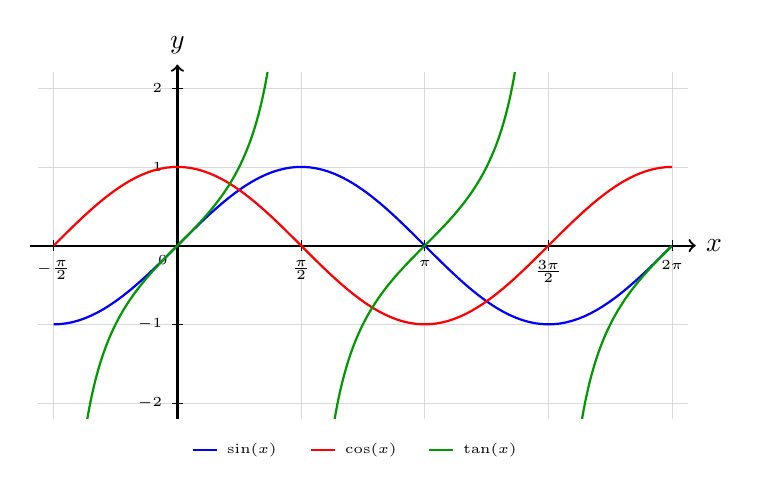
\begin{tikzpicture}
    \draw[very thin, gray!30, xstep={pi/2}, ystep=1] ({-pi/2 - 0.2}, -2.2) grid ({2*pi + 0.2}, 2.2);

    \draw[->, thick] ({-pi/2 - 0.3}, 0) -- ({2*pi + 0.3}, 0) node[right] {$x$};
    \draw[->, thick] (0, -2.2) -- (0, 2.3) node[above] {$y$};

    \draw ({-pi/2}, 2pt) -- ({-pi/2}, -2pt) node[below, font=\tiny] {$-\frac{\pi}{2}$};
    \draw ({pi/2}, 2pt)  -- ({pi/2}, -2pt)  node[below, font=\tiny] {$\frac{\pi}{2}$};
    \draw ({pi}, 2pt)    -- ({pi}, -2pt)    node[below, font=\tiny] {$\pi$};
    \draw ({3*pi/2}, 2pt)-- ({3*pi/2}, -2pt)node[below, font=\tiny] {$\frac{3\pi}{2}$};
    \draw ({2*pi}, 2pt)  -- ({2*pi}, -2pt)  node[below, font=\tiny] {$2\pi$};

    \foreach \y in {-2, -1, 1, 2}
        \draw (2pt, \y) -- (-2pt, \y) node[left, font=\tiny] {$\y$};
    \node[below left, font=\tiny] at (0,0) {$0$};

    \begin{scope}
        \clip ({-pi/2 - 0.2}, -2.2) rectangle ({2*pi + 0.1}, 2.2);

        \draw[thick, blue, domain={-pi/2}:{2*pi}, samples=100] 
            plot (\x, {sin(\x r)});

        \draw[thick, red, domain={-pi/2}:{2*pi}, samples=100] 
            plot (\x, {cos(\x r)});

        \draw[thick, green!60!black, domain=-1.4:1.4, samples=100] 
            plot (\x, {tan(\x r)});
        \draw[thick, green!60!black, domain=1.75:4.55, samples=100] 
            plot (\x, {tan(\x r)});
        \draw[thick, green!60!black, domain=4.9:6.28, samples=50] 
            plot (\x, {tan(\x r)});
    \end{scope}

    \begin{scope}[shift={(0.2, -2.6)}, font=\tiny]
        \draw[thick, blue] (0,0) -- (0.3,0) node[right, black] {$\sin(x)$};
        \draw[thick, red] (1.5,0) -- (1.8,0) node[right, black] {$\cos(x)$};
        \draw[thick, green!60!black] (3.0,0) -- (3.3,0) node[right, black] {$\tan(x)$};
    \end{scope}
\end{tikzpicture}
\end{center}
\end{minipage}

\begin{minipage}{\linewidth}
\Bild Graphen von Trigonometrischen Inversen

\begin{center}
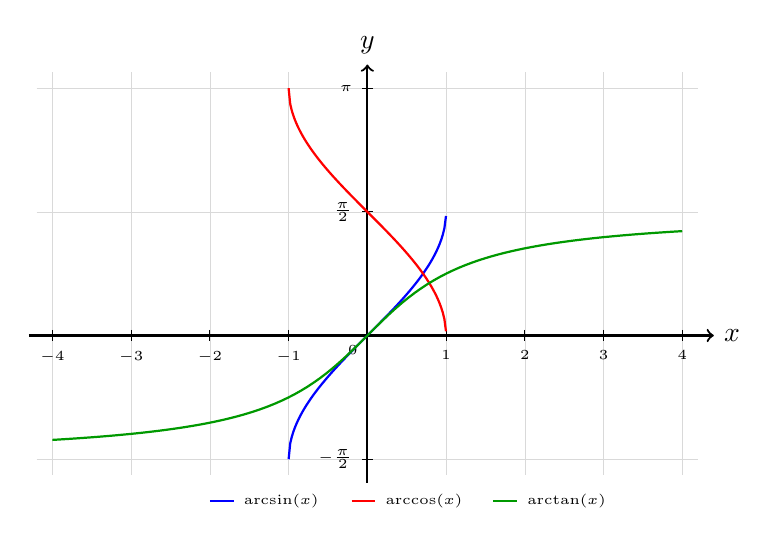
\begin{tikzpicture}
    \draw[very thin, gray!30, xstep=1, ystep={pi/2}] (-4.2, {-pi/2 - 0.2}) grid (4.2, {pi + 0.2});

    \draw[->, thick] (-4.3, 0) -- (4.4, 0) node[right] {$x$};
    \draw[->, thick] (0, {-pi/2 - 0.3}) -- (0, {pi + 0.3}) node[above] {$y$};

    \foreach \x in {-4, -3, -2, -1, 1, 2, 3, 4}
        \draw (\x, 2pt) -- (\x, -2pt) node[below, font=\tiny] {$\x$};

    \draw (2pt, {-pi/2}) -- (-2pt, {-pi/2}) node[left, font=\tiny] {$-\frac{\pi}{2}$};
    \draw (2pt, {pi/2})  -- (-2pt, {pi/2})  node[left, font=\tiny] {$\frac{\pi}{2}$};
    \draw (2pt, {pi})    -- (-2pt, {pi})    node[left, font=\tiny] {$\pi$};
    \node[below left, font=\tiny] at (0,0) {$0$};

    \begin{scope}
        \clip (-4.2, {-pi/2 - 0.2}) rectangle (4.2, {pi + 0.2});

        \draw[thick, blue, domain=-1:1, samples=100] 
            plot (\x, {rad(asin(\x))});

        \draw[thick, red, domain=-1:1, samples=100] 
            plot (\x, {rad(acos(\x))});

        \draw[thick, green!60!black, domain=-4:4, samples=100] 
            plot (\x, {rad(atan(\x))});
    \end{scope}

    \begin{scope}[shift={(-2.0, -2.1)}, font=\tiny]
        \draw[thick, blue] (0,0) -- (0.3,0) node[right, black] {$\arcsin(x)$};
        \draw[thick, red] (1.8,0) -- (2.1,0) node[right, black] {$\arccos(x)$};
        \draw[thick, green!60!black] (3.6,0) -- (3.9,0) node[right, black] {$\arctan(x)$};
    \end{scope}
\end{tikzpicture}
\end{center}
\end{minipage}

\begin{minipage}{\linewidth}
\Bild Graphen von Exponentialfunktionen (und $\frac{1}{x}$ just because)

\begin{center}
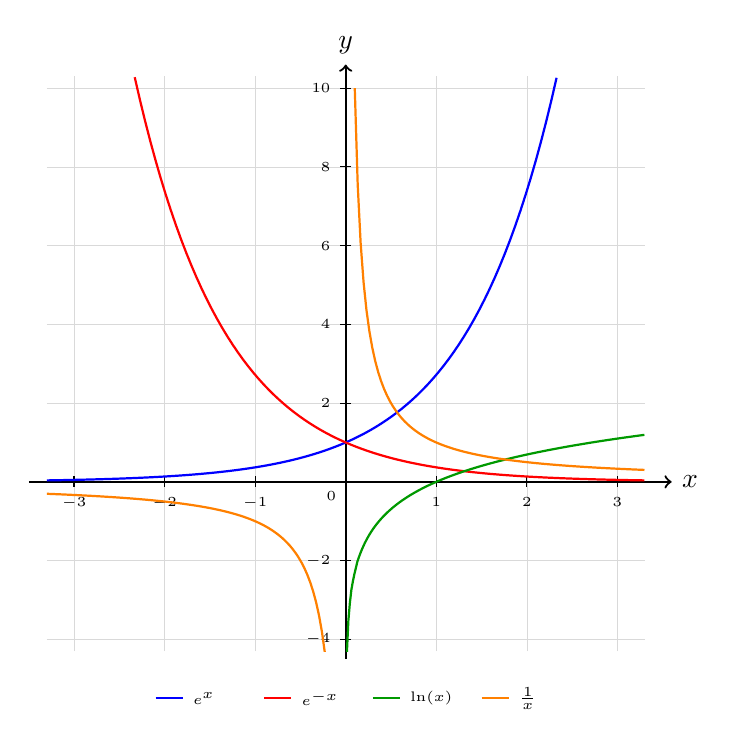
\begin{tikzpicture}[x=1.15cm, y=0.5cm]
    % Grid matching xstep = 1 and ystep = 2
    \draw[very thin, gray!30, xstep=1, ystep=2] (-3.3, -4.3) grid (3.3, 10.3);

    % Axes
    \draw[->, thick] (-3.5, 0) -- (3.6, 0) node[right] {$x$};
    \draw[->, thick] (0, -4.5) -- (0, 10.6) node[above] {$y$};

    % X-Axis Ticks (Steps of 1 from -3 to 3)
    \foreach \x in {-3, -2, -1, 1, 2, 3}
        \draw (\x, 2pt) -- (\x, -2pt) node[below, font=\tiny] {$\x$};

    % Y-Axis Ticks (Steps of 2 from -4 to 10)
    \foreach \y in {-4, -2, 2, 4, 6, 8, 10}
        \draw (2pt, \y) -- (-2pt, \y) node[left, font=\tiny] {$\y$};
    \node[below left, font=\tiny] at (0,0) {$0$};

    % Clip plot region
    \begin{scope}
        \clip (-3.3, -4.3) rectangle (3.3, 10.3);

        % 1. e^x (Blue)
        \draw[thick, blue, domain=-3.3:2.33, samples=100] 
            plot (\x, {exp(\x)});

        % 2. e^-x (Red)
        \draw[thick, red, domain=-2.33:3.3, samples=100] 
            plot (\x, {exp(-\x)});

        % 3. ln(x) (Green)
        \draw[thick, green!60!black, domain=0.013:3.3, samples=200] 
            plot (\x, {ln(\x)});

        % 4. 1/x (Orange) - Split domain to avoid x = 0 asymptote
        \draw[thick, orange, domain=-3.3:-0.1, samples=100] 
            plot (\x, {1/\x});
        \draw[thick, orange, domain=0.1:3.3, samples=100] 
            plot (\x, {1/\x});
    \end{scope}

    % Legend
    \begin{scope}[shift={(0.0, -5.5)}, font=\tiny]
        \draw[thick, blue] (-2.1,0) -- (-1.8,0) node[right, black] {$e^x$};
        \draw[thick, red] (-0.9,0) -- (-0.6,0) node[right, black] {$e^{-x}$};
        \draw[thick, green!60!black] (0.3,0) -- (0.6,0) node[right, black] {$\ln(x)$};
        \draw[thick, orange] (1.5,0) -- (1.8,0) node[right, black] {$\frac{1}{x}$};
    \end{scope}

\end{tikzpicture}
\end{center}
\end{minipage}

\begin{minipage}{\linewidth}
\Tab Wichtige Grenzwerte

\begin{tabular}{l c r}
    $\lim f(x)$ & Grenzwert $L$ & Bedingung \\
    \hline
    $\lim\limits_{n\to\infty} \frac{\ln n}{n}$ & $0$ & \\[1ex]
    $\lim\limits_{n\to\infty} \sqrt[n]{n}$ & $1$ & \\[1ex]
    $\lim\limits_{n\to\infty} \sqrt[n]{x}$ & $1$ & $x > 0$ \\[1ex]
    $\lim\limits_{n\to\infty} \left(1 + \frac{x}{n}\right)^n$ & $e^x$ & $x \in \mathbb{R}$ \\[1ex]
    $\lim\limits_{n\to\infty} \frac{x^n}{n!}$ & $0$ & $x \in \mathbb{R}$ \\[0.5ex]
    \hline
    $\lim\limits_{n\to\infty} x^n$ & $0$ & $|x| < 1$ \\[1ex]
    $\lim\limits_{n\to\infty} \frac{n^k}{a^n}$ & $0$ & $a > 1, k \in \mathbb{R}$ \\[1ex]
    $\lim\limits_{n\to\infty} \frac{a^n}{n!}$ & $0$ & $a > 0$ \\[1ex]
    $\lim\limits_{n\to\infty} \frac{n!}{n^n}$ & $0$ & \\[1ex]
    $\lim\limits_{n\to\infty} \sqrt[n]{a^n + b^n}$ & $\max(a, b)$ & $a, b \ge 0$ \\
    \hline
    $\lim\limits_{x\to 0} \frac{\sin x}{x}$ & $1$ & $x \neq 0$ \\[1ex]
    $\lim\limits_{x\to 0} \frac{1 - \cos x}{x^2}$ & $\frac{1}{2}$ & $x \neq 0$ \\[1ex]
    $\lim\limits_{x\to 0} \frac{e^x - 1}{x} = \lim\limits_{x\to 0} \frac{e^x}{x + 1}$ & $1$ & $x \neq 0$ \\[1ex]
    $\lim\limits_{x\to 0} \frac{\ln(1 + x)}{x}$ & $1$ & $x > -1, x \neq 0$ \\[1ex]
    $\lim\limits_{x\to 0} \frac{(1 + x)^k - 1}{x}$ & $k$ & $k \in \mathbb{R}, x \neq 0$ \\[0.5ex]
    \hline
    $\lim\limits_{x\to 0^+} x^x$ & $1$ & \\[1ex]
    $\lim\limits_{x\to 0^+} x^a \ln x$ & $0$ & $a > 0$ \\[1ex]
    $\lim\limits_{x\to\infty} \frac{(\ln x)^k}{x^a}$ & $0$ & $a > 0, k \in \mathbb{R}$
\end{tabular}
\end{minipage}

\begin{minipage}{\linewidth}
\Tab Wichtige Maclaurin-Reihen

\begin{tabular}{l c c r}
    $f(x)$ & Entwicklung & Summenform & Bedingung \\
    \hline
    $e^x$ & $1 + x + \frac{x^2}{2!} + \dots$ & $\sum_{k=0}^\infty \frac{x^k}{k!}$ & $x \in \mathbb{R}$ \\[1ex]
    $\cos x$ & $1 - \frac{x^2}{2!} + \frac{x^4}{4!} - \dots$ & $\sum_{k=0}^\infty (-1)^k \frac{x^{2k}}{(2k)!}$ & $x \in \mathbb{R}$ \\[1ex]
    $\sin x$ & $x - \frac{x^3}{3!} + \frac{x^5}{5!} - \dots$ & $\sum_{k=0}^\infty (-1)^k \frac{x^{2k+1}}{(2k+1)!}$ & $x \in \mathbb{R}$ \\[1ex]
    $\cosh x$ & $1 + \frac{x^2}{2!} + \frac{x^4}{4!} + \dots$ & $\sum_{k=0}^\infty \frac{x^{2k}}{(2k)!}$ & $x \in \mathbb{R}$ \\[1ex]
    $\sinh x$ & $x + \frac{x^3}{3!} + \frac{x^5}{5!} + \dots$ & $\sum_{k=0}^\infty \frac{x^{2k+1}}{(2k+1)!}$ & $x \in \mathbb{R}$ \\[1ex]
    \hline
    $\frac{1}{1-x}$ & $1 + x + x^2 + \dots$ & $\sum_{k=0}^\infty x^k$ & $|x| < 1$ \\[1ex]
    $\frac{1}{1+x}$ & $1 - x + x^2 - \dots$ & $\sum_{k=0}^\infty (-1)^k x^k$ & $|x| < 1$ \\[1ex]
    $\ln(1+x)$ & $x - \frac{x^2}{2} + \frac{x^3}{3} + \dots$ & $\sum_{k=1}^\infty (-1)^{k-1} \frac{x^k}{k}$ & $-1 < x \le 1$ \\[1ex]
    $\arctan x$ & $x - \frac{x^3}{3} + \frac{x^5}{5} - \dots$ & $\sum_{k=0}^\infty (-1)^k \frac{x^{2k+1}}{2k+1}$ & $|x| \le 1$ \\[1ex]
    $(1+x)^\alpha$ & $1 + \alpha x + \dots$ & $\sum_{k=0}^\infty \binom{\alpha}{k} x^k$ & $|x| < 1$ \\
\end{tabular}
\end{minipage}

\begin{minipage}{\linewidth}
\Tab Ableitungen und Stammfunktionen

\begin{tabular}{l c r}
    $f(x)$ & $f'(x)$ & $\int f(x) \, dx (+ C)$ \\
    \hline
    $x^n \ (n \neq -1)$ & $n x^{n-1}$ & $\frac{x^{n+1}}{n+1}$ \\[1ex]
    $\sqrt{x}$ & $\frac{1}{2\sqrt{x}}$ & $\frac{2}{3}x\sqrt{x}$ \\[1ex]
    $\sqrt[n]{x}$ & $\frac{1}{n\sqrt[n]{x^{n-1}}}$ & $\frac{n}{n+1}x\sqrt[n]{x}$ \\[1ex]
    $\frac{1}{x}$ & $-\frac{1}{x^2}$ & $\ln|x|$ \\[1ex]
    $e^x$ & $e^x$ & $e^x$ \\[1ex]
    $a^x$ & $a^x \ln a$ & $\frac{a^x}{\ln a}$ \\[1ex]
    $\ln x$ & $\frac{1}{x}$ & $x \ln x - x$ \\[0.5ex]
    \hline
    $\sin x$ & $\cos x$ & $-\cos x$ \\[1ex]
    $\cos x$ & $-\sin x$ & $\sin x$ \\[1ex]
    $\tan x$ & $\sec^2 x$ & $-\ln|\cos x|$ \\[1ex]
    $\sec x$ & $\sec x \tan x$ & $\ln|\sec x + \tan x|$ \\[1ex]
    $\csc x$ & $-\csc x \cot x$ & $-\ln|\csc x + \cot x|$ \\[1ex]
    $\cot x$ & $-\csc^2 x$ & $\ln|\sin x|$ \\
    \hline
    $\arcsin x$ & $\frac{1}{\sqrt{1-x^2}}$ & $x \arcsin x + \sqrt{1-x^2}$ \\[1ex]
    $\arccos x$ & $-\frac{1}{\sqrt{1-x^2}}$ & $x \arccos x - \sqrt{1-x^2}$ \\[1ex]
    $\arctan x$ & $\frac{1}{1+x^2}$ & $x \arctan x - \frac{1}{2}\ln(1+x^2)$ \\[0.5ex]
    \hline
    $\sinh x$ & $\cosh x$ & $\cosh x$ \\[1ex]
    $\cosh x$ & $\sinh x$ & $\sinh x$ \\[1ex]
    $\tanh x$ & $\operatorname{sech}^2 x$ & $\ln(\cosh x)$ \\
\end{tabular}
\end{minipage}


\end{multicols*}

\pagebreak

\clearpage

\end{document}
